\documentclass[12pt]{report}

\usepackage[a4paper,
			inner = 35mm,
			outer = 25mm,
			top = 25mm,
			bottom = 25mm]{geometry}
\usepackage{lmodern}
\usepackage[magyar]{babel}
\usepackage[utf8]{inputenc}
\usepackage[T1]{fontenc}
\usepackage[hidelinks]{hyperref}
\usepackage{graphicx}
\usepackage{amssymb}
\usepackage{setspace}
\usepackage[nottoc,numbib]{tocbibind}
\usepackage{amsthm}
\usepackage{minted}
\usepackage{mdframed}
\usepackage{etoolbox}



% \setcounter{secnumdepth}{3}
\onehalfspacing

\newtheorem{mydef}{Definició}
\newtheorem{mytetel}{Tétel}
\newtheorem{mylemma}{Lemma}

\BeforeBeginEnvironment{minted}{\begin{mdframed}[backgroundcolor=bg, hidealllines=true]}
\AfterEndEnvironment{minted}{\end{mdframed}}

\newcommand{\cmd}[1]{\colorbox{gray!10}{\strut #1}}

\definecolor{bg}{rgb}{0.95,0.95,0.95}
\newminted[mintedJson]{js}{breaklines, breaksymbolleft=\quad}
\newminted[mintedBash]{bash}{breaklines, breaksymbolleft=\quad}



\begin{document}

\begin{titlepage}
	\begin{center}
		\vspace*{1cm}
		
		\textbf{\LARGE 
			Forgalom igény tudatos hálózat tervezés minimális torlódással és úthosszal
		}
	
	
		\vspace{0.5cm}
	
		\textbf{\normalsize Tudáskezelő rendszerek III. labor összefoglaló}
		
		\vfill
		
		\Large Szecsődi Imre
		
		\vspace{2.8cm}
		
		\the\year
		
	\end{center}
\end{titlepage}

\tableofcontents
	
\chapter{Bevezetés}


\section{Labor célja}

A labor célja a korábban már bemutatott cikk\cite{avin_demand-aware_nodate} hálózat építése.
Az eredeti cikkben a fák építésére az Egofa algoritmus volt használva, a labor keretén belül azt a felvetést vizsgáltam meg, hogy lehet-e jobb algoritmust találni fa építésre, mint az Egofa. 
A különböző módszerek az eredetihez hasonlóan véletlenszerűen generált gráfokra vannak tesztelve. 
Az új módosított algoritmusok eredménye az eredetivel voltak összehasonlítva.

\section{Laborban megvalósított munka}

A labor ideje alatt a már elkészült keretrendszer adta az alapot, ami segítségével tesztelhető a szerzők által felvázolt és három saját fejlesztésű algoritmus is.
A keretrendszer Python \cite{noauthor_python_nodate} nyelven íródott.
Egy véletlen gráfok generálására a NetworkX külső csomag volt használva\cite{noauthor_networkx_nodate}.
Az adatok elemzése pedig RapidMiner-ben történt\cite{noauthor_lightning_nodate}.

\chapter{Modell}

\section{Az új algoritmusok}

\subsection{Egobalance}

Az első algoritmus majdnem teljes mértékben megegyezik az eredetivel.
A cikk szerzői az Egofa algoritmus vázlatos összefoglalásában használtak egy csere lépést.
A csere lépés lényege, hogy mikor megépítettük a fákat, azután ki kell iktatni a direkt kapcsolatokat a magas-magas csomópontok között.
Mikor a segítő nincs a fában, ott nincs semmi egyéb tenni valónk, mivel egy csere történik, és a csomópont gyerekei nem vándorolnak sehova.
Ezzel ellentétben, mikor a segítő pont is része a fának, akkor két lehetőségünk van, ha a segítő közelebb van a gyökérhez akkor töröljük a magas pontot, ha pedig a magas pont van feljebb, akkor a segítő átveszi a helyét, majd töröljük a magast.

A említett algoritmus egyik lényeges része, hogy mi történik a gyerekekkel, mivel vagy a segítő vagy a magas pont gyerekeit vissza kell kapcsolni a fára.
Az eredeti implementációban a törölt csomópont szülőjére lett rákapcsolva a nehezebb gyerek, és a maradék fa pedig hasonló elven, addig hozta fel a nehezebb pontot még minden hiányzó belső csomópont nem lett kitöltve. 
Az Egobalance logaritmus a függő pontok újra elhelyezését az Egofára bízza, azaz újra elosztásra kerülnek.
Ezzel elméletben mindig arra törekszik az algoritmus, hogy optimális legyen torlódásra nézve az új fa.
Lényegi különbség úthossznál jelentkezik az eredetivel szemben.

\subsection{Huffman fa}

A eddigi két algoritmus az Egofát használta, ami optimális torlódásra nézve, de mivel a hálózat nem csak torlódás szempontjából van vizsgálva ezért meg kell vizsgálni a másik aspektusát is az optimális úthosszt.
A Huffman kódolásnál használt fa tulajdonsága, hogy átlagosan rövidek legyenek a gyakoriságot tekintve.
A cl-Dan probléma is ezt a tényezőt használja, ezért kitűnően lehet használni ezt a fát a hálózat alapjának.
Egyetlen probléma a Huffman fával az, hogy a belső csomópontok nem tartalmaznak számunkra hasznos információt.
Ezért szükséges egy kiegészítő lépés, ami segítségével belső pontok is ki lesznek töltve hasznos információval, azaz esetünkben csomópontokkal, amik maguk is végpontok, mint a levelek.

Az algoritmus első része teljesen megegyezik a Huffman kódolással.
Rendezzük sorba növekedően a pontokat, és kettesével vonjuk össze őket, még nem kapunk egy teljes fát.
Egy kis kiegészítés itt, hogy hasonlóan mint az Egofáknál, a legfelső szinten \(n\) darab csúcsot tudunk a gyökérre kapcsolni, ami maga a forrás csomópont.
Az összes többi alacsonyabb pont pedig marad bináris.

A belső pontok kitöltése pedig a következő módon történik:
\begin{enumerate}
	\item A gyökér csomóponthoz kapcsolódó ágakon szedjük össze a leveleket
	\item Ezeket a leveleket sorfolytonosan kapcsoljuk rá ág gyökér csomópontjára, az előtt említett bináris módon
\end{enumerate}
 
Felmerülhet a kérdés, hogy miért nem a legnehezebb levél jön fel mindig?
Ez azért van, mert a Huffman kódolásnál megtörténik az az eset, hogy két csomópont összesített értéke megegyezik egy harmadikkal.
Ez olyan fát eredményez, ahol bal oldalon egy nehéz csomópont és jobb oldalon fában két könnyű csomópont szerepel.
A naiv megoldás esetén ez azt eredményezi, hogy az egy nehéz lesz a belső csomópont, és az ág ahonnan jött megüresedik.
A pont levelei nem fognak ágat változtatni, annak ellenére, hogy megüresedett az egyik feljebb, ezért hosszú egyenes utak jöhetnek létre.
Ennek kiküszöbölésére van a sorfolytonos algoritmus, ahol garantálni lehet, hogy fa egyik belső csomópontja sem marad kitöltetlen levél nélkül.

\subsection{Sorfolytonos fa}

Mint láthattuk korábban a Huffman fánál láttuk a levelek felfelé mozgatását sorfolytonosan, itt hasonló az elv.
Lényegi különbséggel, hogy itt még a Huffman kódolási algoritmust kihagyjuk, és egyenest sorfolytonosan rakjuk már eleve fel csomópontokat.
Ezzel mindig a legkisebb fákat kapjuk, de ez a torlódást egyáltalán nem veszi figyelembe.

\chapter{Megvalósítás}


\section{Adatszerkezetek}

A modell alapját pár egyszerű alaptípus adja. Ezek rendre a következők:
\begin{itemize}
	\item \textbf{Vertex} - az általános gráf csúcspont
	\item \textbf{Node} - az \textit{Egófák} készítésekor használt csomópontok amik tartalmazzák a valószínűségét annak, hogy a forrás csomópont mekkora valószínűséggel fog kommunikálni a másik \textit{Node} csomóponttal
	\item \textbf{HuffmanDanNode} - a Huffman fa csomópontjait reprezentáló osztály, minden tulajdonsága megvan mint a Node-nak, csak még kiegészül egy útvonallal, amit a Huffman fa építése után lesz meghatározva
	\item \textbf{Edge} - az gráf csomópontjait reprezentáló él, ami \textit{Vertexet} vár paraméterként, és tárolja a valószínűséget, hasonlóan mint a \textit{Node}
	\item \textbf{Tree} - ami adja az alapját majd a útvonal tervezési sémának. A fának két fajtája lehet:
	\begin{itemize}
		\item \textbf{BinTree} - a kettő fokú fa
		\item \textbf{EgoTree} - a $\Delta$ fokú fa, ahol a gyökérnek legfeljebb $\Delta$ levele lehet, és a levelek pedig \textit{BinTree} típúsuak.
		\item \textbf{HuffmanDanTree} - a $\Delta$ fokú Huffman fa, ahol a belső csomópontok tudnak kitöltetlenek is lenni
	\end{itemize}

	
\end{itemize}
	
\section{Modell}

A \textbf{Network} osztály megváltozott az előző megvalósításhoz képest.
Absztrakt osztályra lett átalakítva, a belőle leszármazó osztályok valósítják meg a különböző algoritmusokat.
A leszármazott osztályoknak egyetlen függvényt kell csak megvalósítani, ami a fa építései stratégiát tartalmazza.
Ennek segítségével nagyon egyszerűen lehet új algoritmust illeszteni a már meglévő rendszerhez.

A bemeneti konfiguráció kiegészült még egy új gráf típussal, a csillag gráf.
Csillag gráfnak nevezzük azt a gráfot, ahol az összes pont egy ponthoz kapcsolódik.
A konfiguráció további egységesítésen esett át, minden véletlen gráf szerkezete megegyezik, ami a következő:

\begin{itemize}
	\item \cmd{graph} - Gráf típusa, lehetséges értékek:
	\begin{itemize}
		\item \cmd{barabasei-albert} - Barabási-Albert gráf
		\item \cmd{erdos-renyi} - Erdős-Rényi gráf
		\item \cmd{star} - Csillag gráf
	\end{itemize}
	
	\item \cmd{vertex\textunderscore num} - Csomópontok száma
	\item \cmd{dan} - A maximális fokszám a magas fokú csúcsokra
	\item \cmd{constant} - Constans érték ami a gráf paraméterét adja, ezek rendre
	
	\begin{itemize}
		\item Barabási-Albert gráf esetén ez azt határozza meg, hogy az új csomópont mennyi másikhoz kapcsolódjon, ami már benne van a gráfban
		\item Erdős-Rényi gráf esetén a valószínűség számításánál használjuk a következő képletben  \[p = constant \cdot \frac{1}{vertex\_num}\]
		\item Csillag gráf esetén pedig a csillagok számát adjuk meg
	\end{itemize}
\end{itemize}

\chapter{Teszt eredmények}

\section{Tesztelés menete}

A tesztelés során mindegyik véletlen gráfok volt használva, és minden algoritmus ugyanazon a bemeneti mátrixon dolgozott a egyértelmű összehasonlítás érdekében. 
A mérések a konstans alapján lettek kiértékelve, mivel az a fő érték, ami alapján változik a gráf ritkasága.
A skálázhatóság tesztelésére különböző számú csúcspont volt használva, ezek rendre: 11, 15, 35, 50, 75, 100, 125, 150, 175 és 200.
A skálázhatósághoz még hozzátartozik a maximum fokszám, hogy mennyi gráf csúcs tud egyszerre kommunikálni, ezért az is meg van adva.
A valóságban van egy fizikai határ, hogy mennyi kliens tud csatlakozni egyszerre, ezért az értékek így lettek megválasztva, 10, 16, 24 és 48.
A konkrét számú csomópont mellett még volt vizsgálva az is, hogy valóságban mekkora szorzóra van szükségünk, mivel a cikk ad egy magas felső becslést ami $\Delta=12\rho$.
Ezért a teszt során figyelve volt az ajánlott fokszám és a tényleges is.
Az ajánlott fokszám értékei a következők voltak $\Delta\in[1\rho, 2\rho, 4\rho, 6\rho, 8\rho, 10\rho, 12\rho]$.
Az így megadott paraméterek alapján 52800 teszt lett lefuttatva.



\section{Eredmények}

\subsection{Átlag Súlyozott úthossz}


\begin{figure}[h]
	\begin{center}
		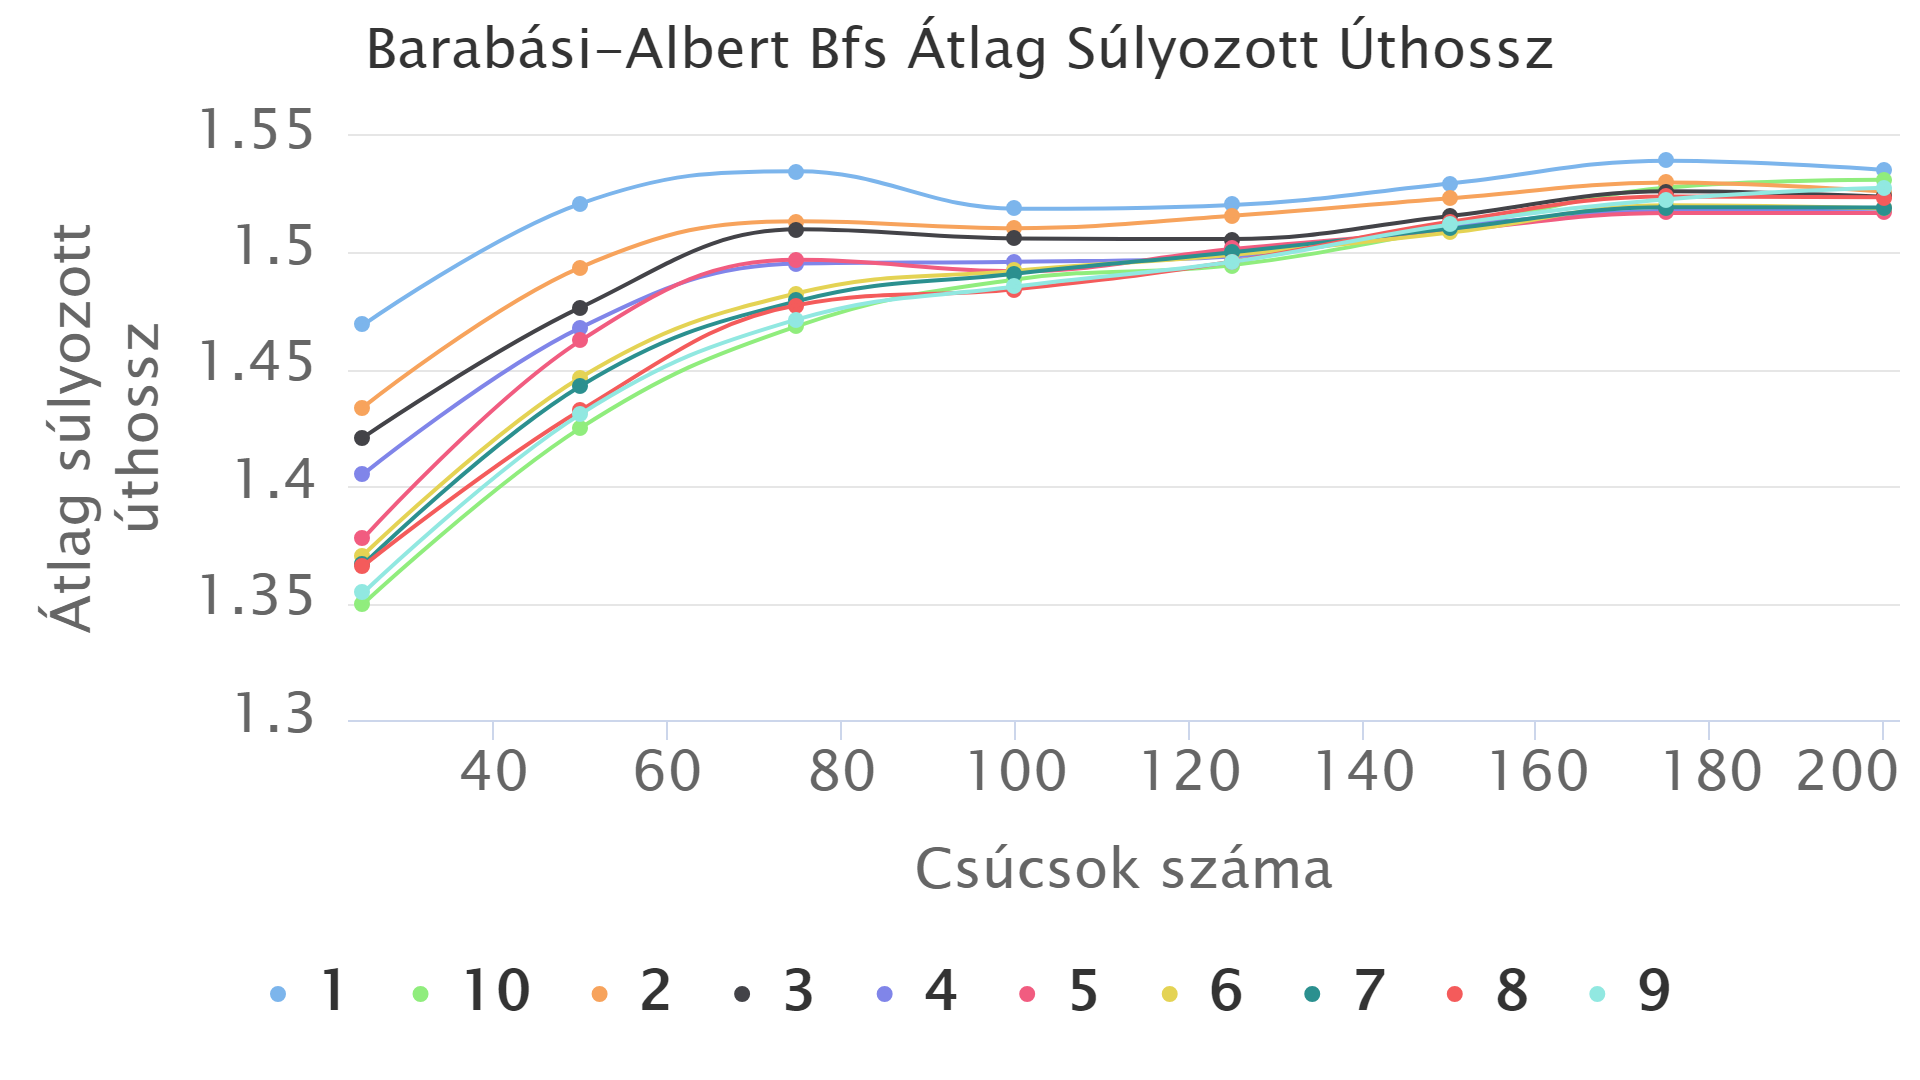
\includegraphics[width=0.49\linewidth]{pictures/barabasi_avg_len_bfs.png}
		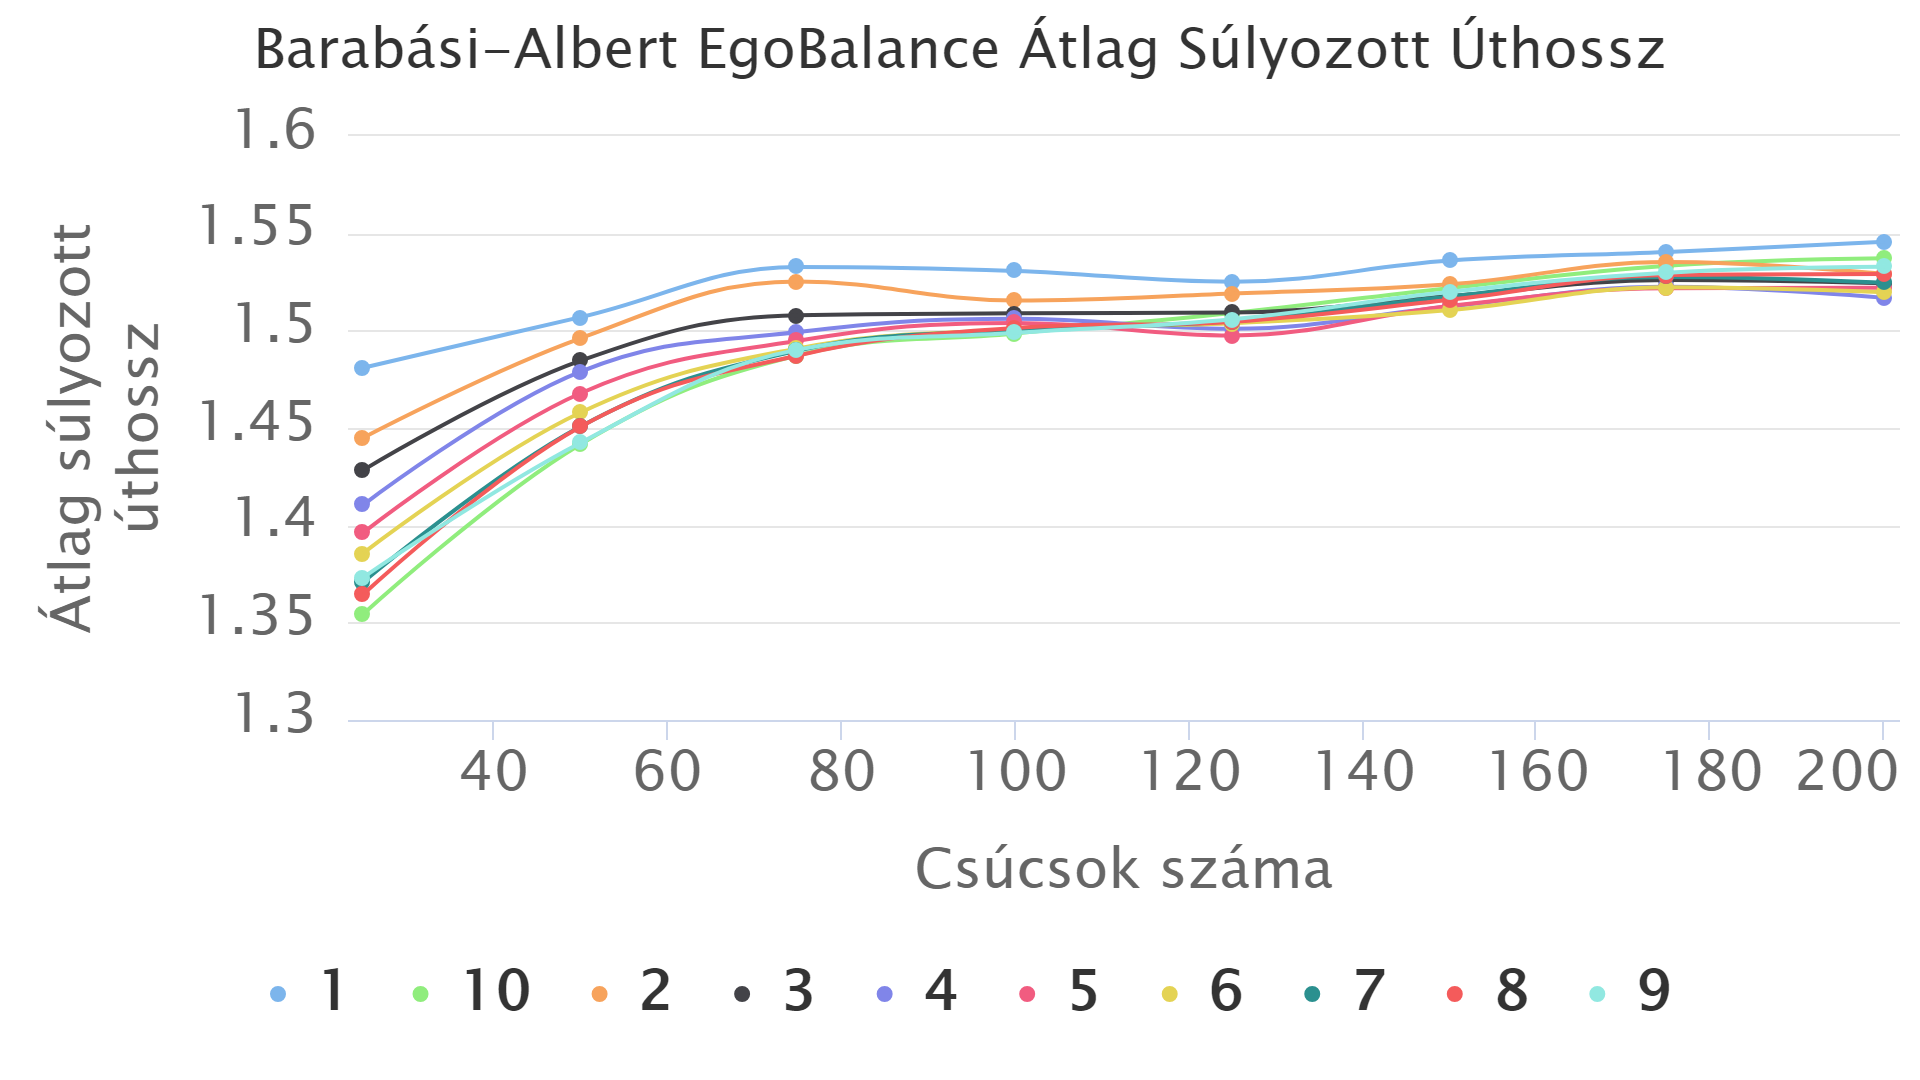
\includegraphics[width=0.49\linewidth]{pictures/barabasi_avg_len_egobalance.png}
		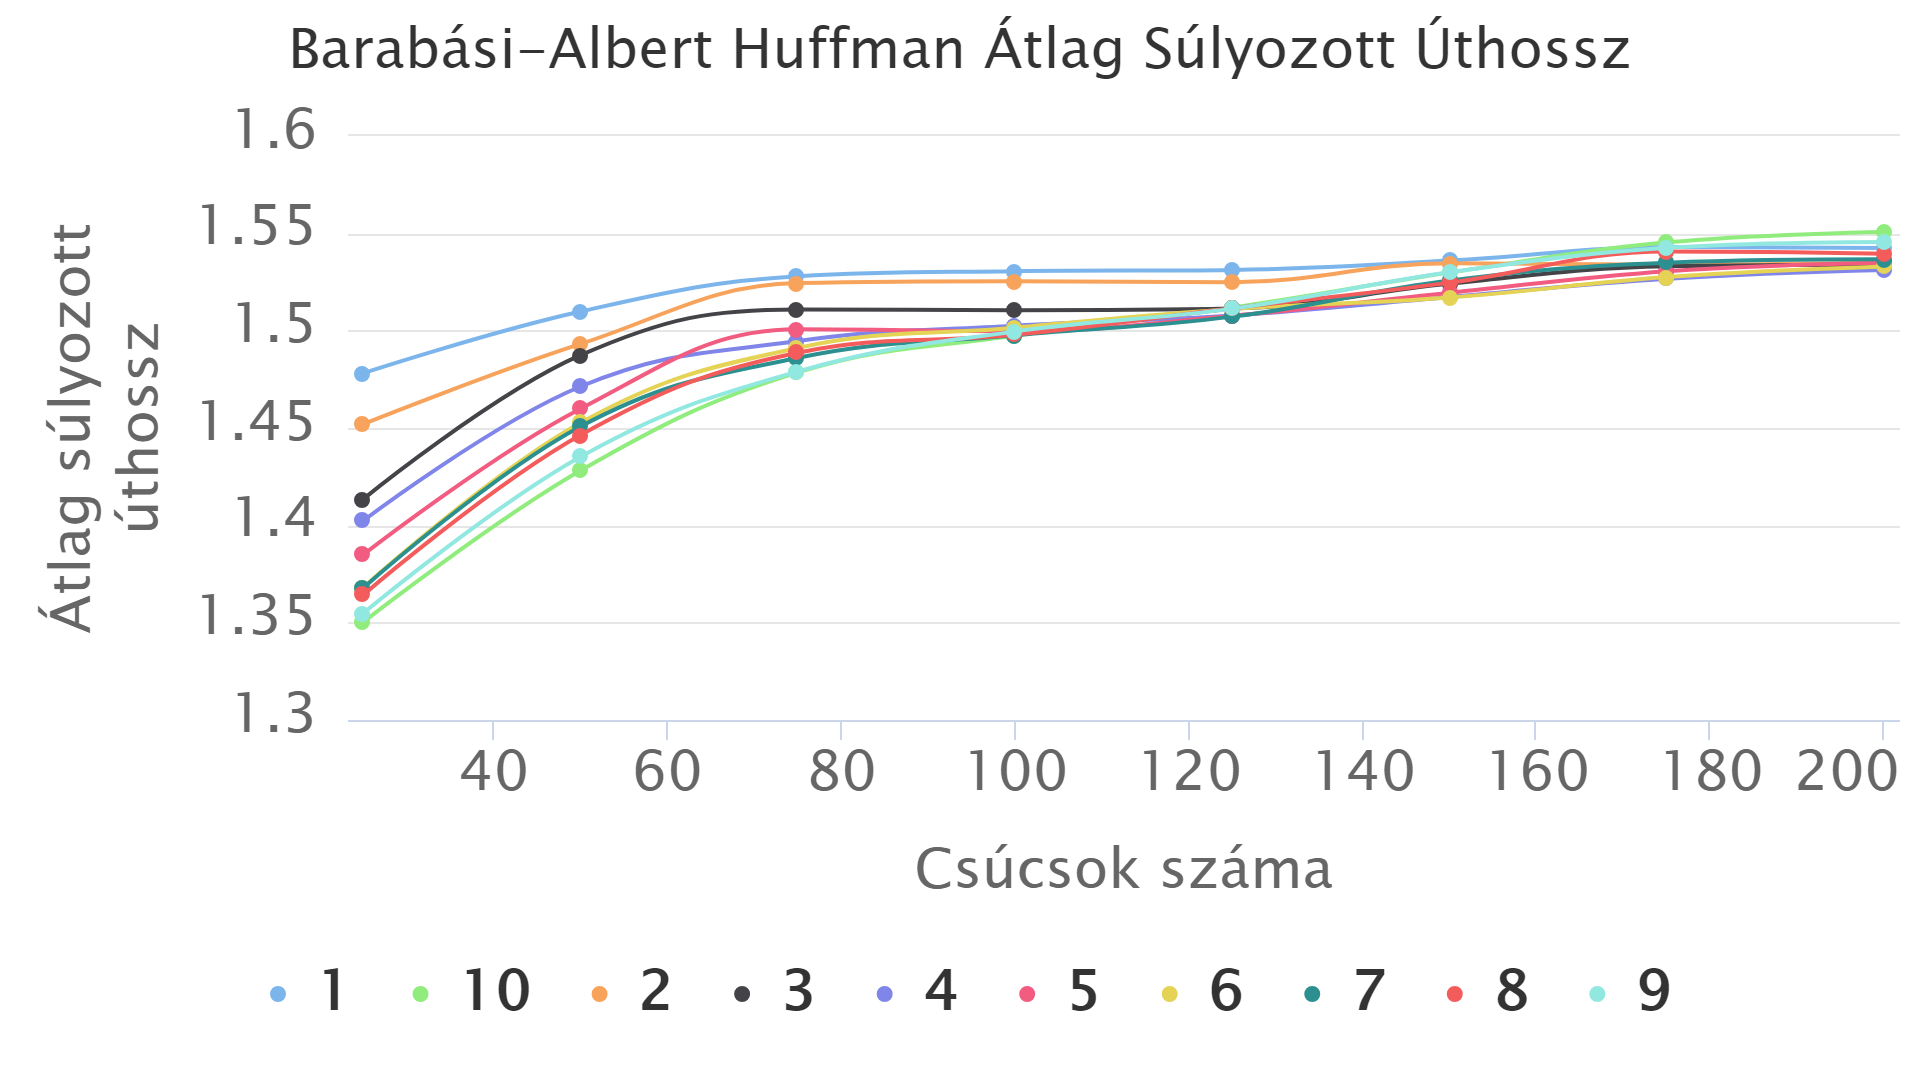
\includegraphics[width=0.49\linewidth]{pictures/barabasi_avg_len_huffman.png}
		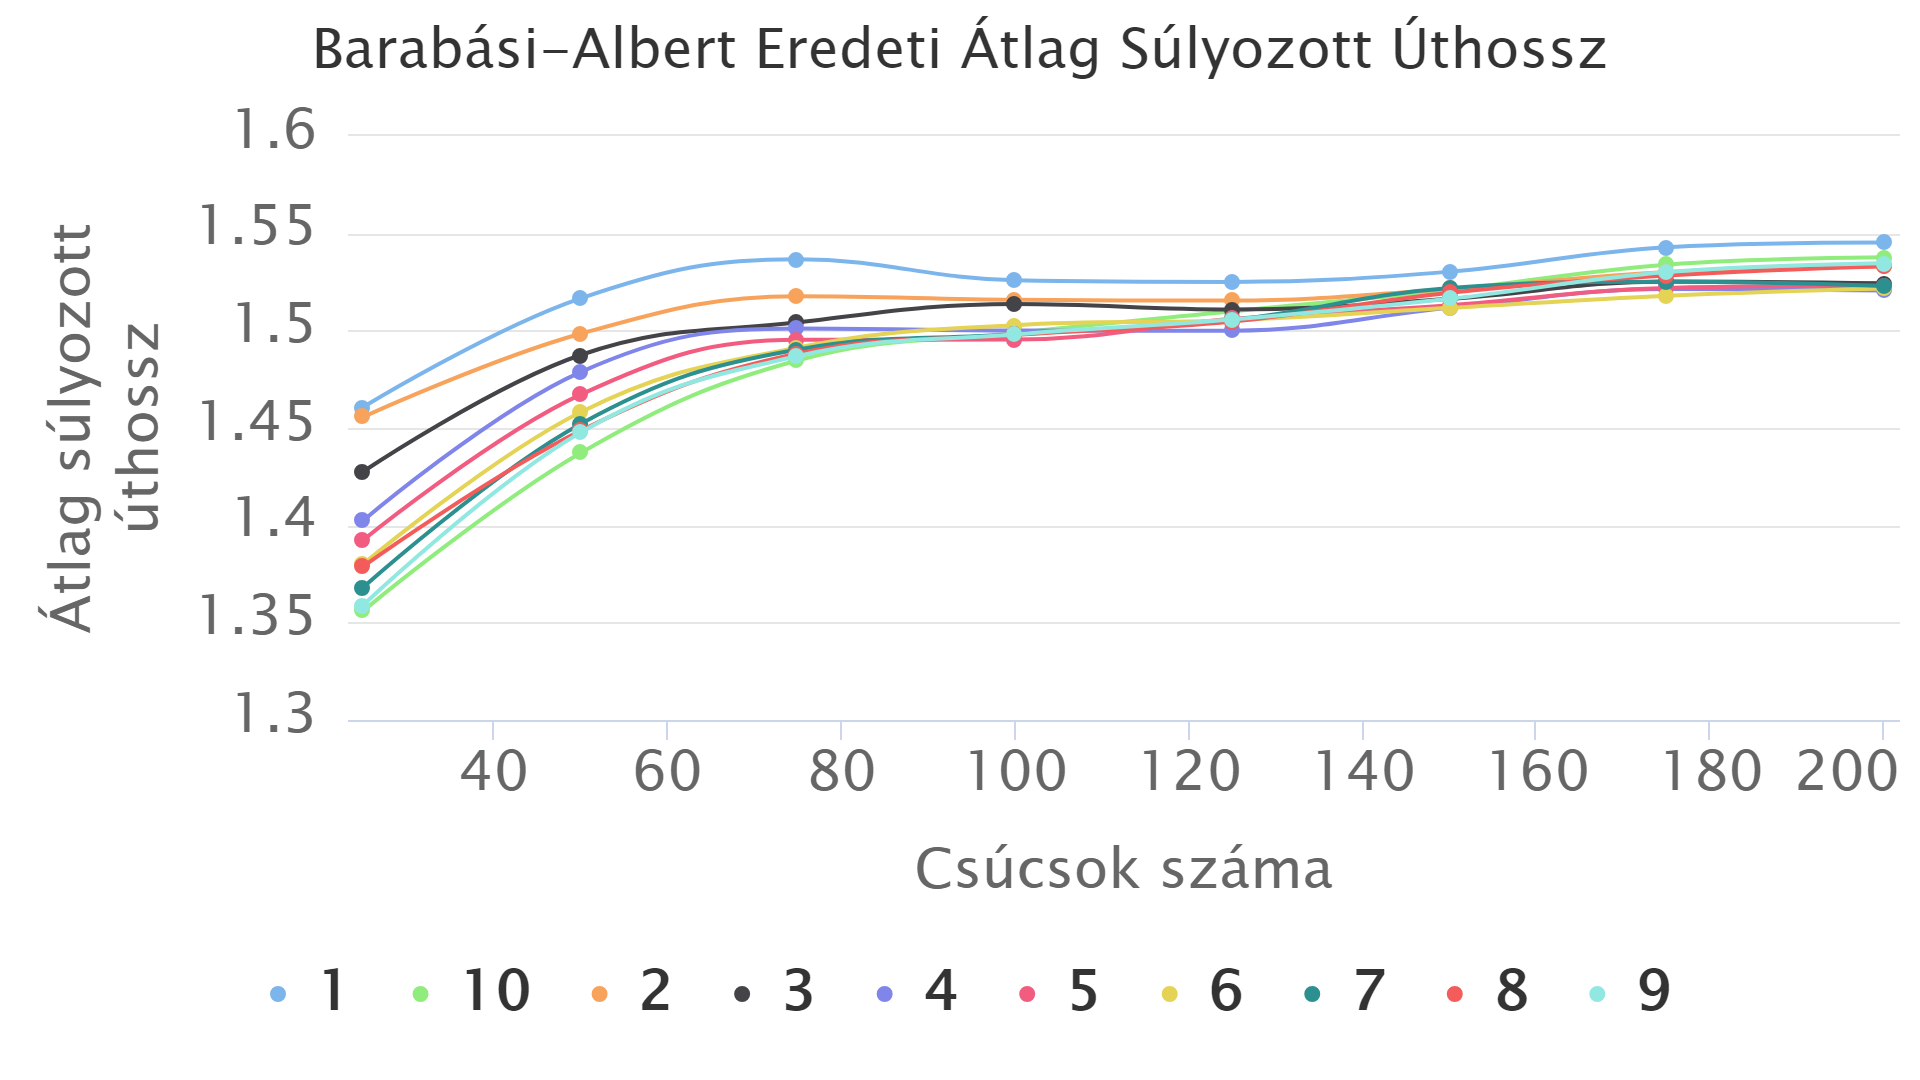
\includegraphics[width=0.49\linewidth]{pictures/barabasi_avg_len_original.png}
		\caption{Átlag súlyozott úthossz Barabási-Albert Gráf}
	\end{center}
\end{figure}


\begin{figure}[h]
	\begin{center}
		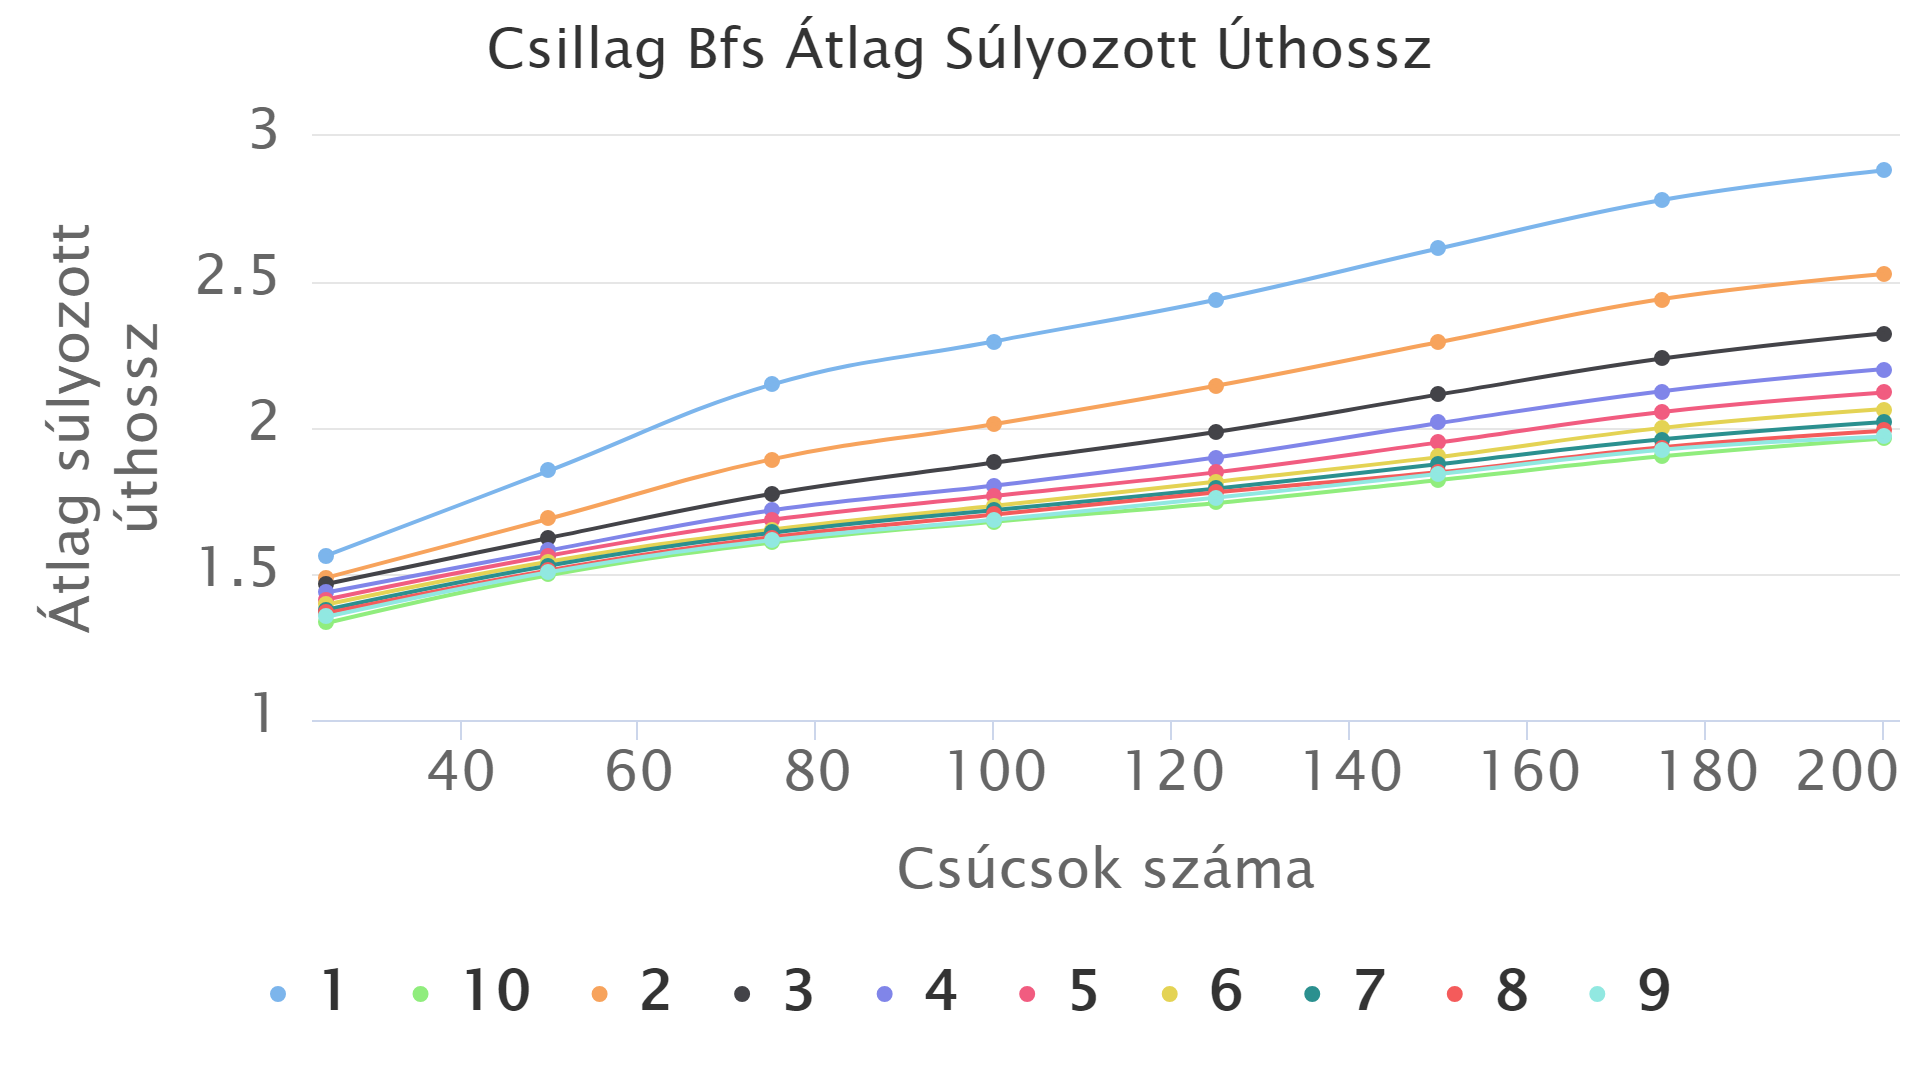
\includegraphics[width=0.49\linewidth]{pictures/star_avg_len_bfs.png}
		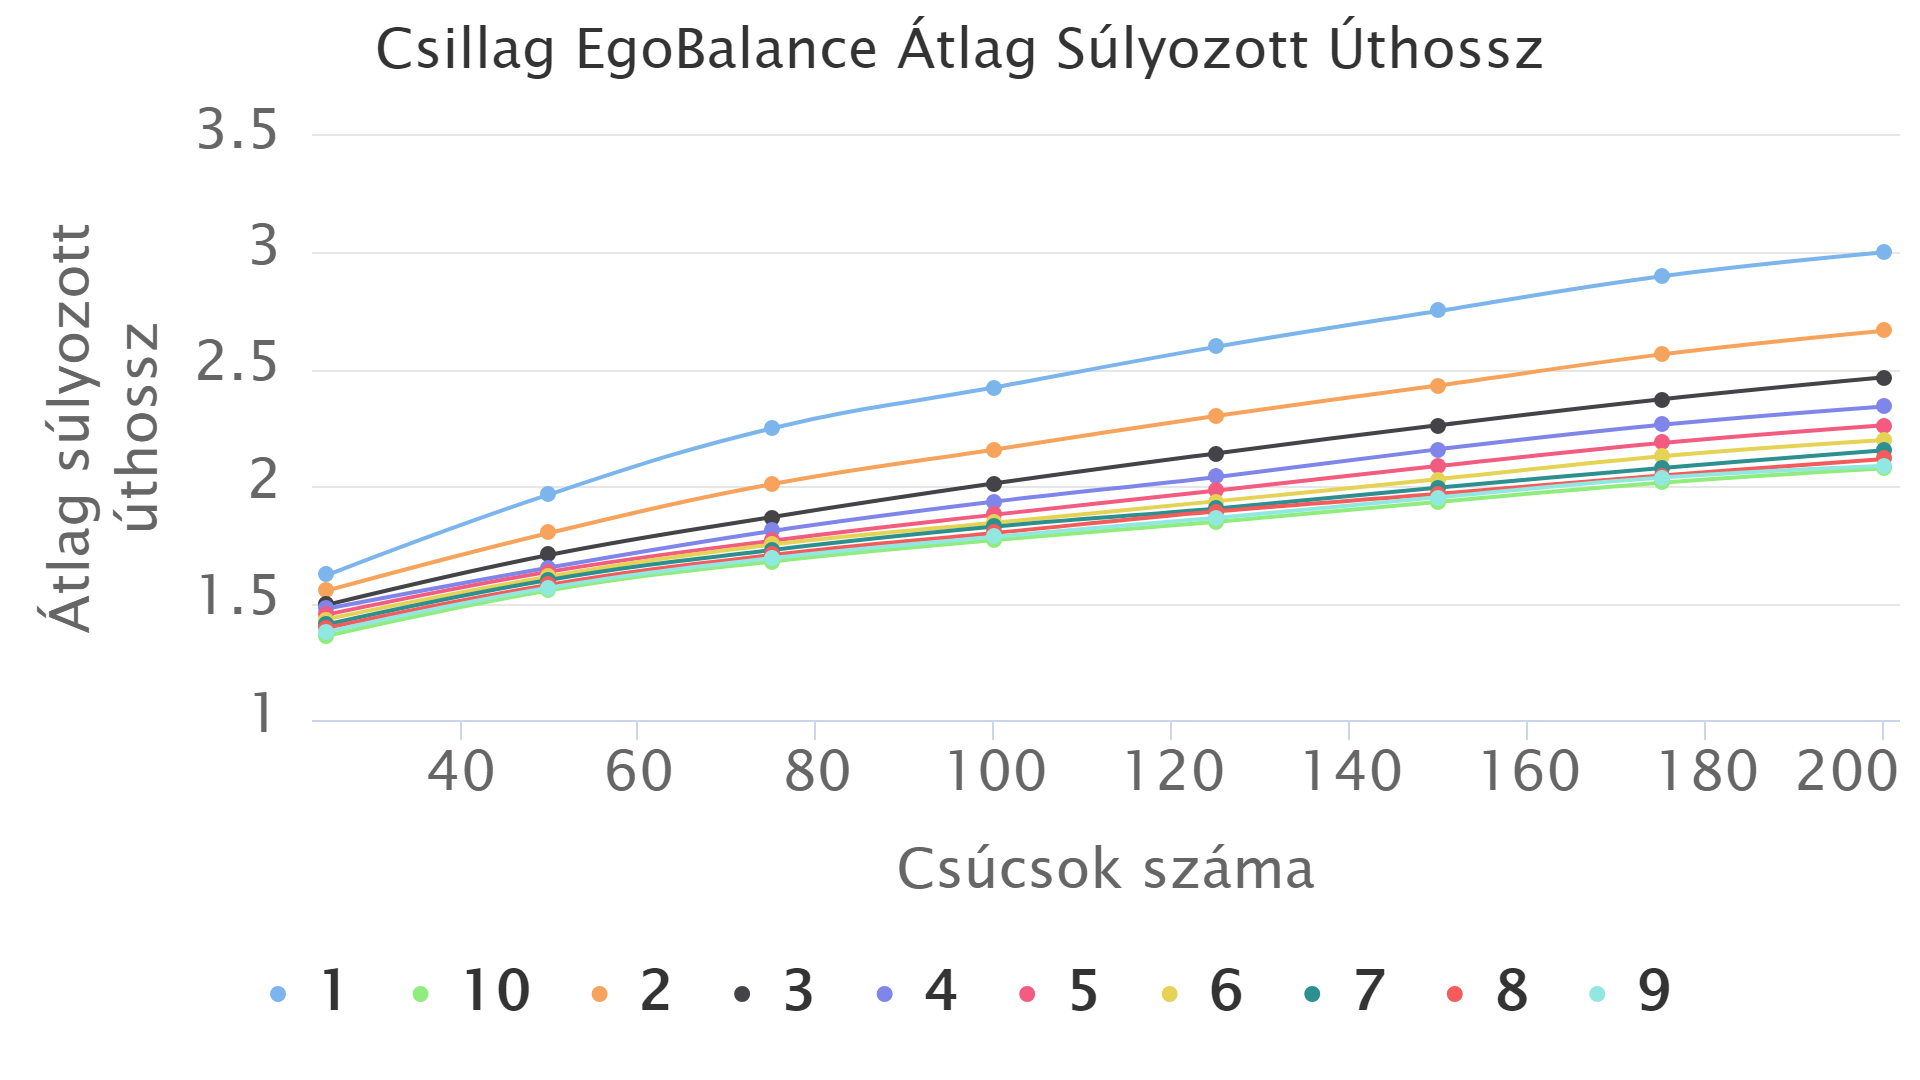
\includegraphics[width=0.49\linewidth]{pictures/star_avg_len_egobalance.png}
		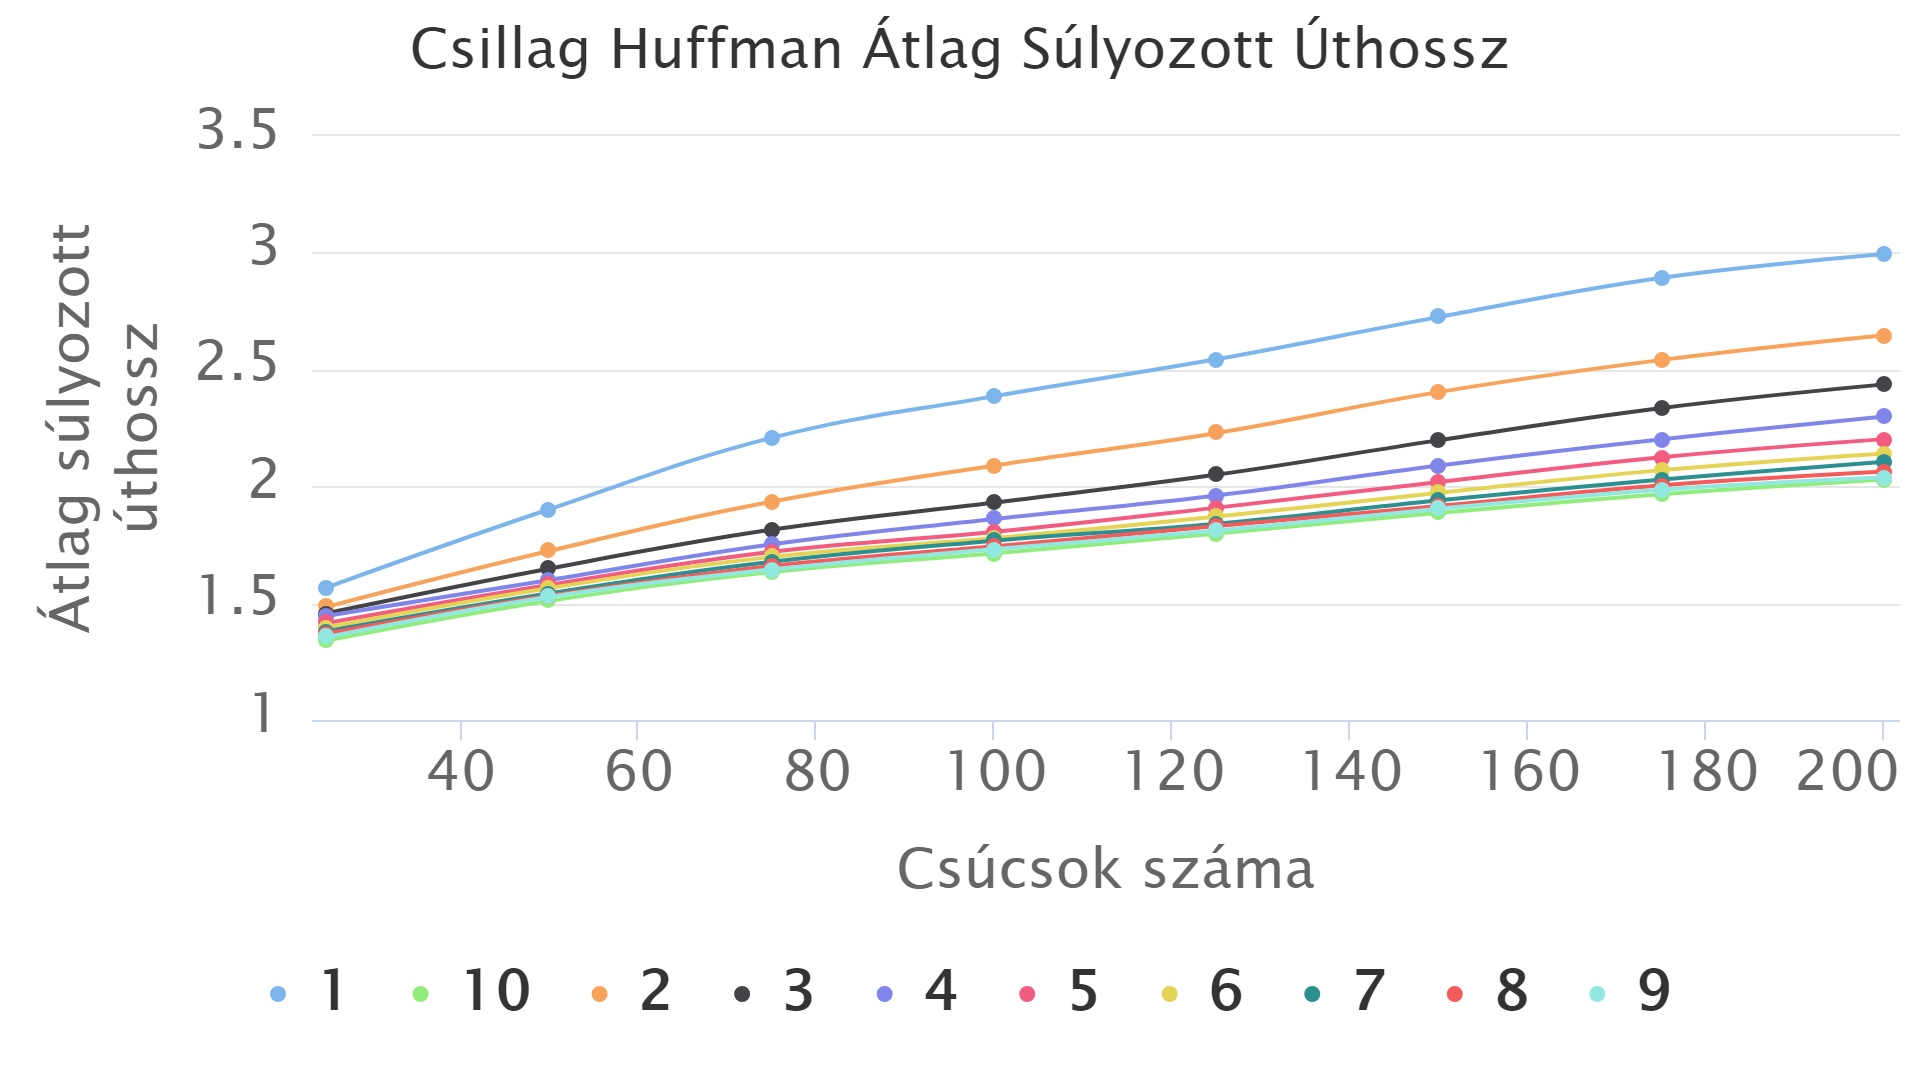
\includegraphics[width=0.49\linewidth]{pictures/star_avg_len_huffman.png}
		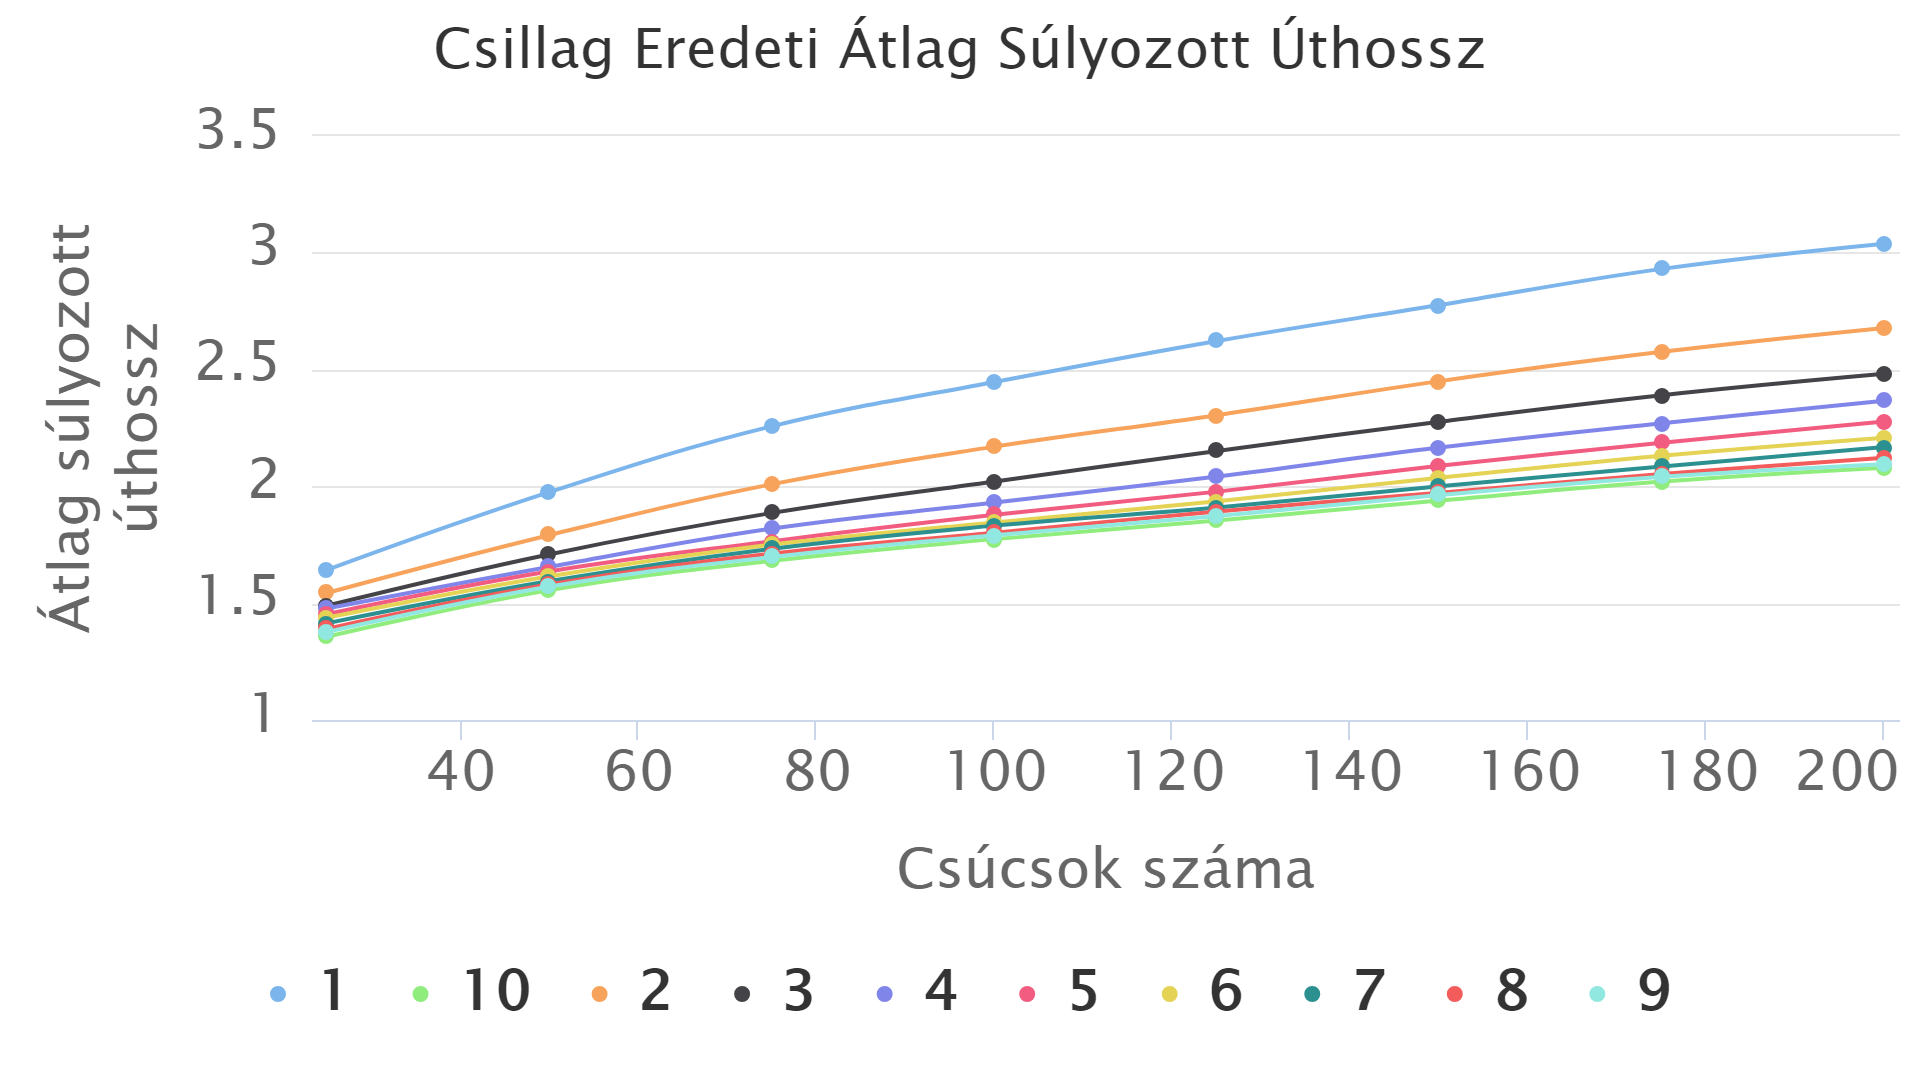
\includegraphics[width=0.49\linewidth]{pictures/star_avg_len_original.png}
		\caption{Átlag súlyozott úthossz Csillag gráf}
	\end{center}
\end{figure}

\begin{figure}[h]
	\begin{center}
		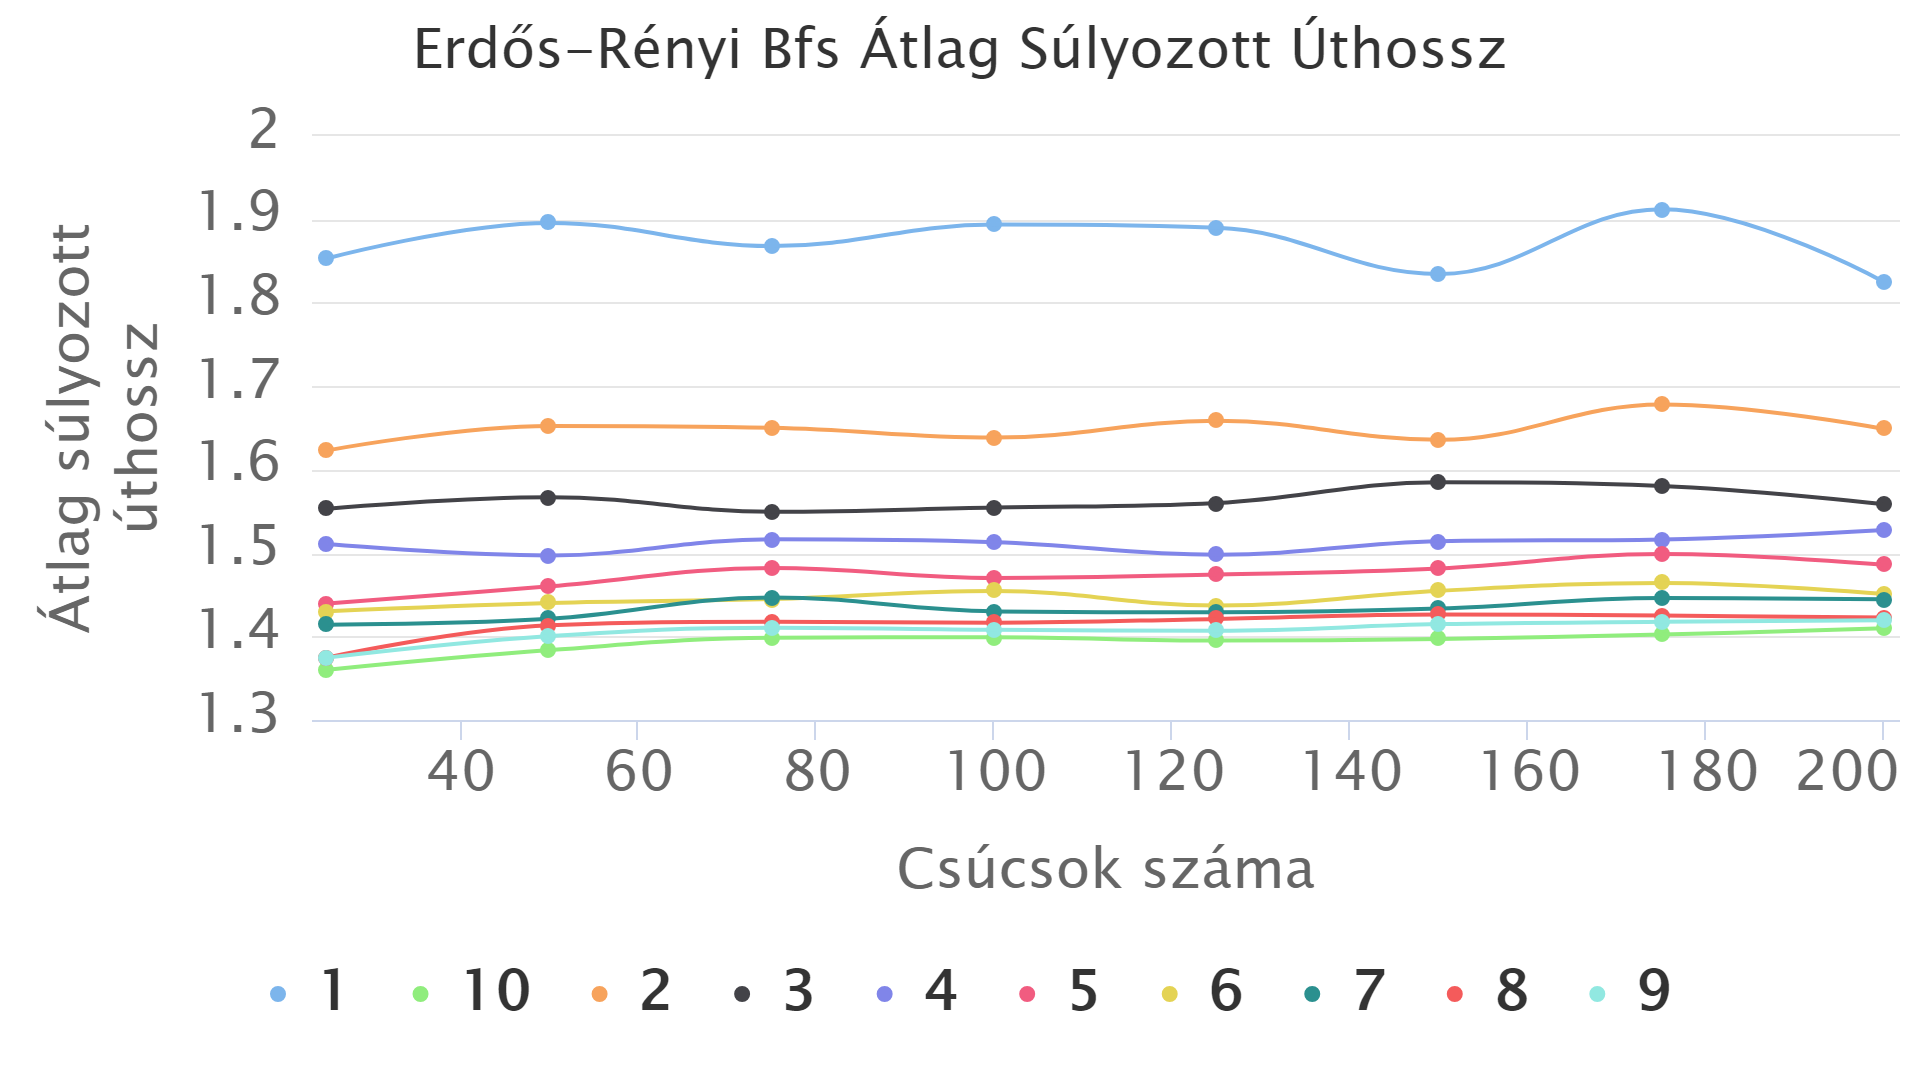
\includegraphics[width=0.49\linewidth]{pictures/erdos_avg_len_bfs.png}
		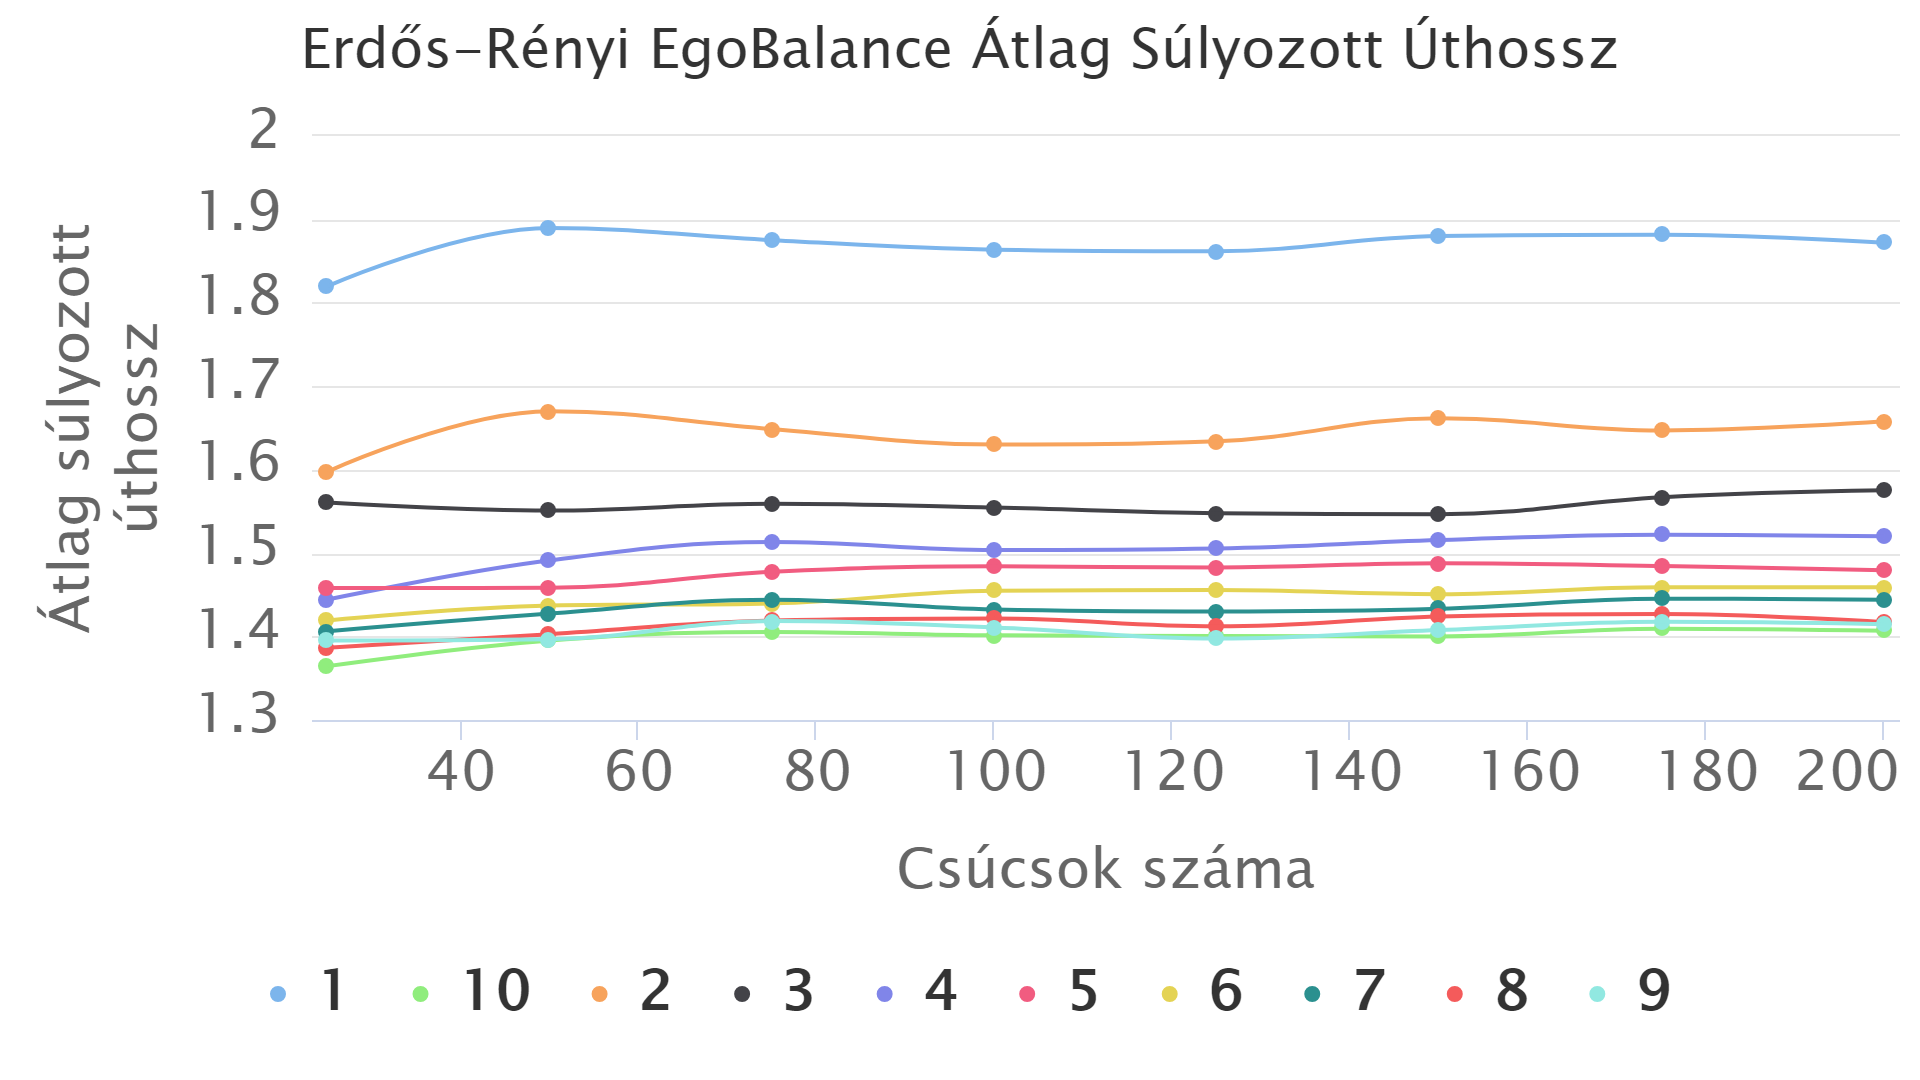
\includegraphics[width=0.49\linewidth]{pictures/erdos_avg_len_egobalance.png}
		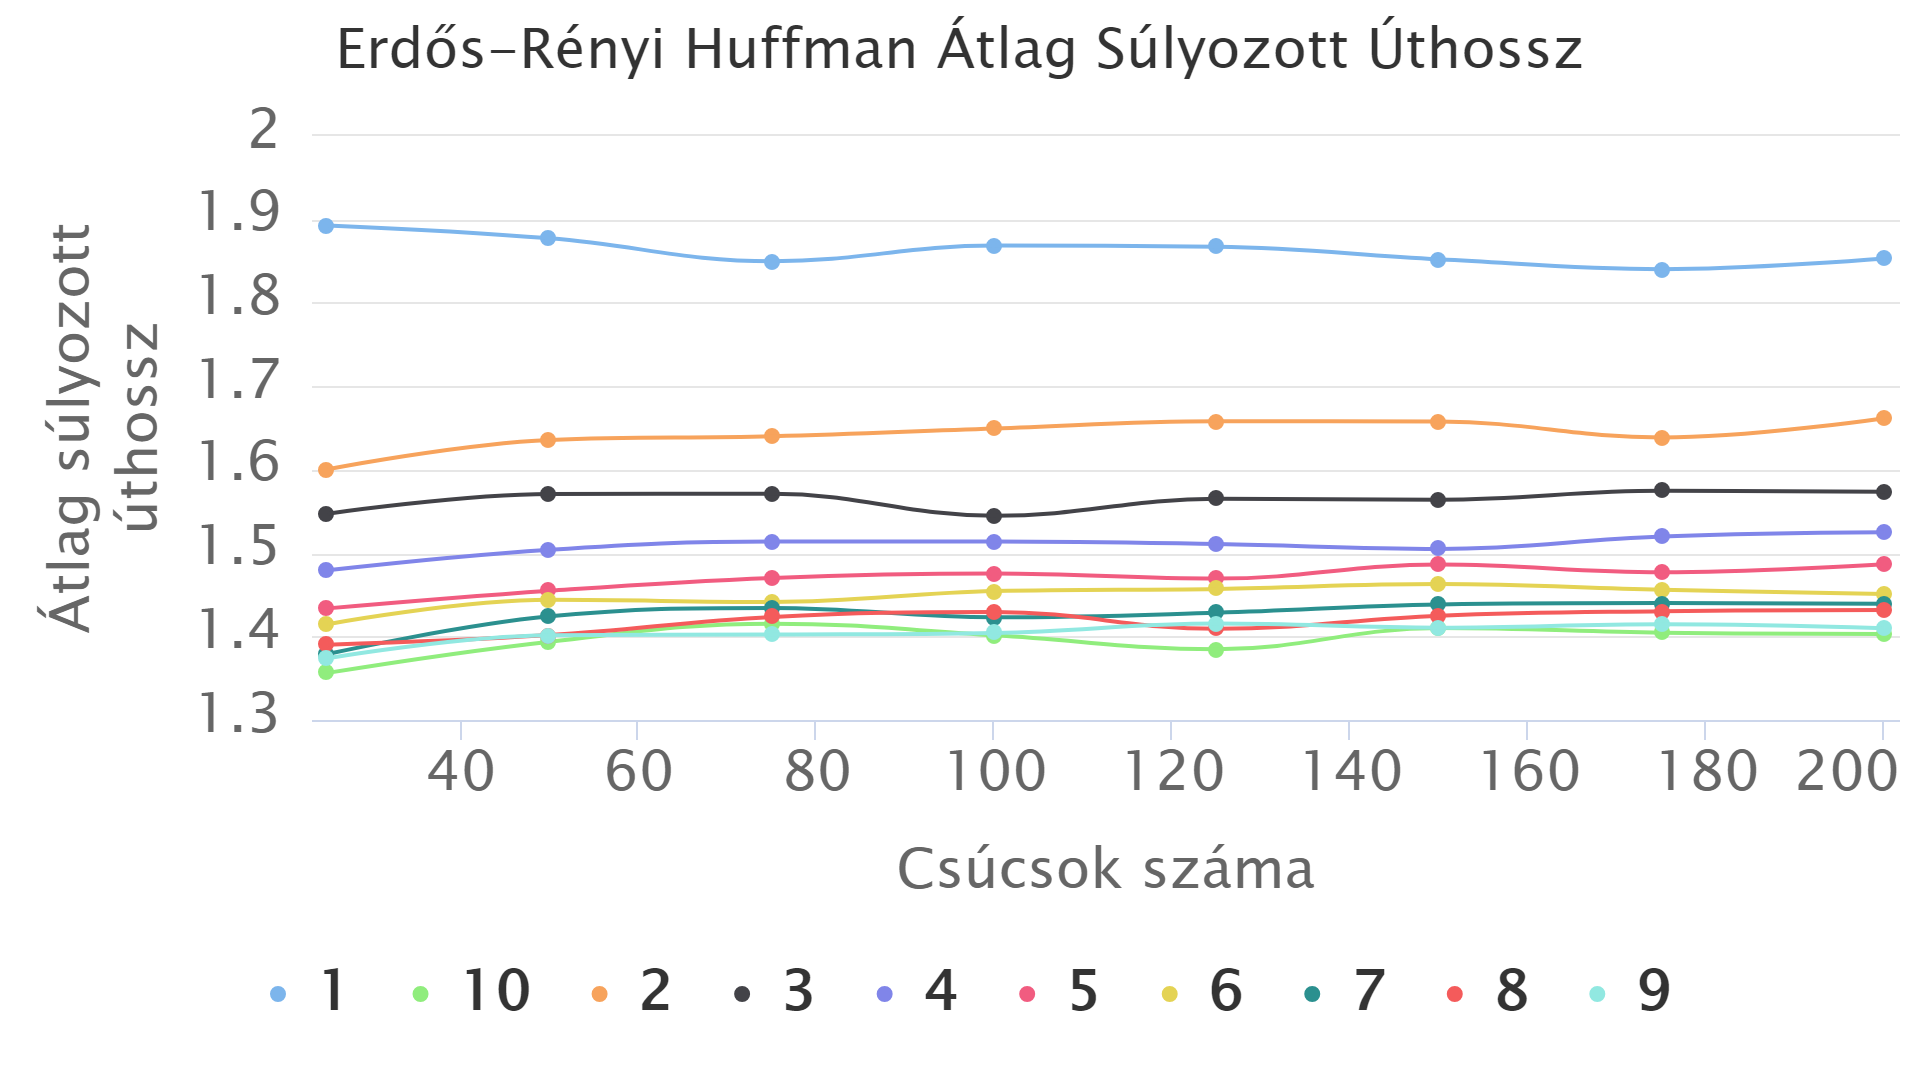
\includegraphics[width=0.49\linewidth]{pictures/erdos_avg_len_huffman.png}
		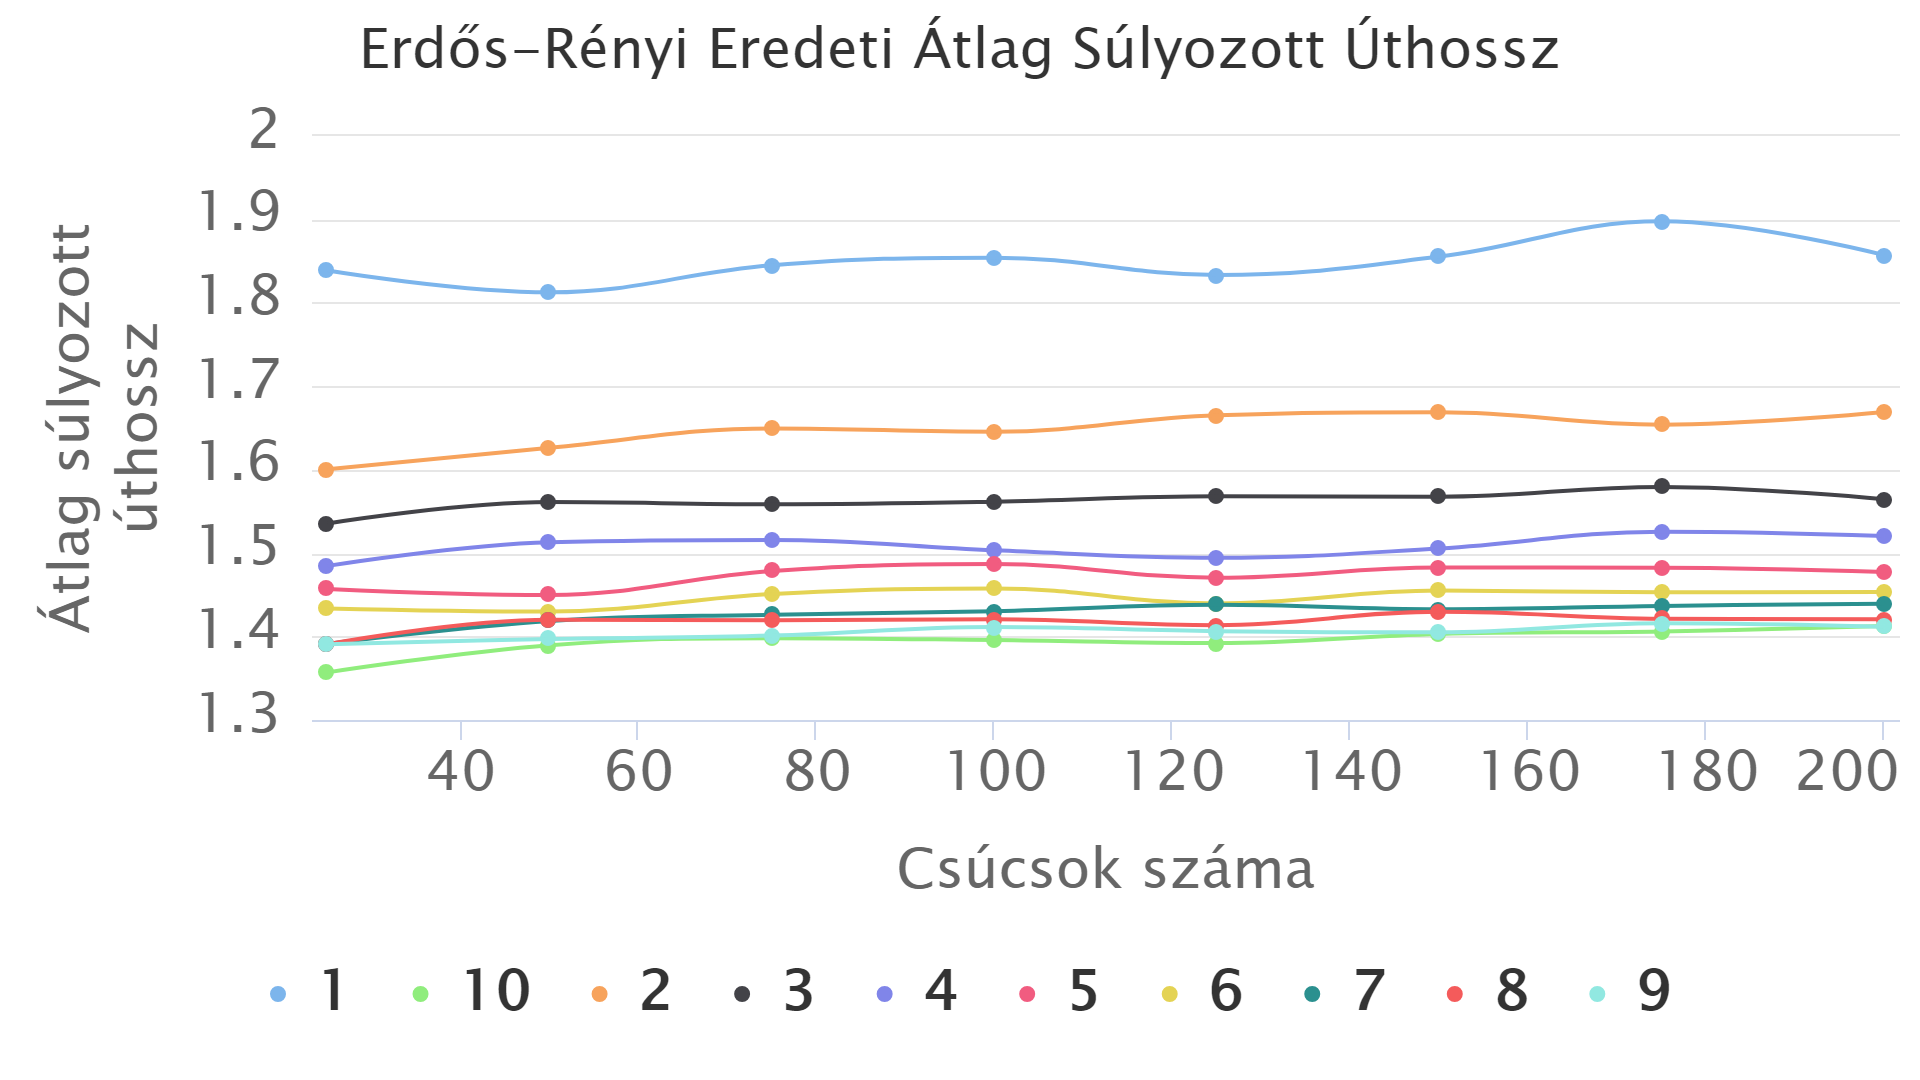
\includegraphics[width=0.49\linewidth]{pictures/erdos_avg_len_original.png}
		\caption{Átlag súlyozott úthossz Erdős-Rényi Gráf}
		\label{avg-len}
	\end{center}
\end{figure}

\subsection{Átlag torlódás}

\begin{figure}[h]
	\begin{center}
		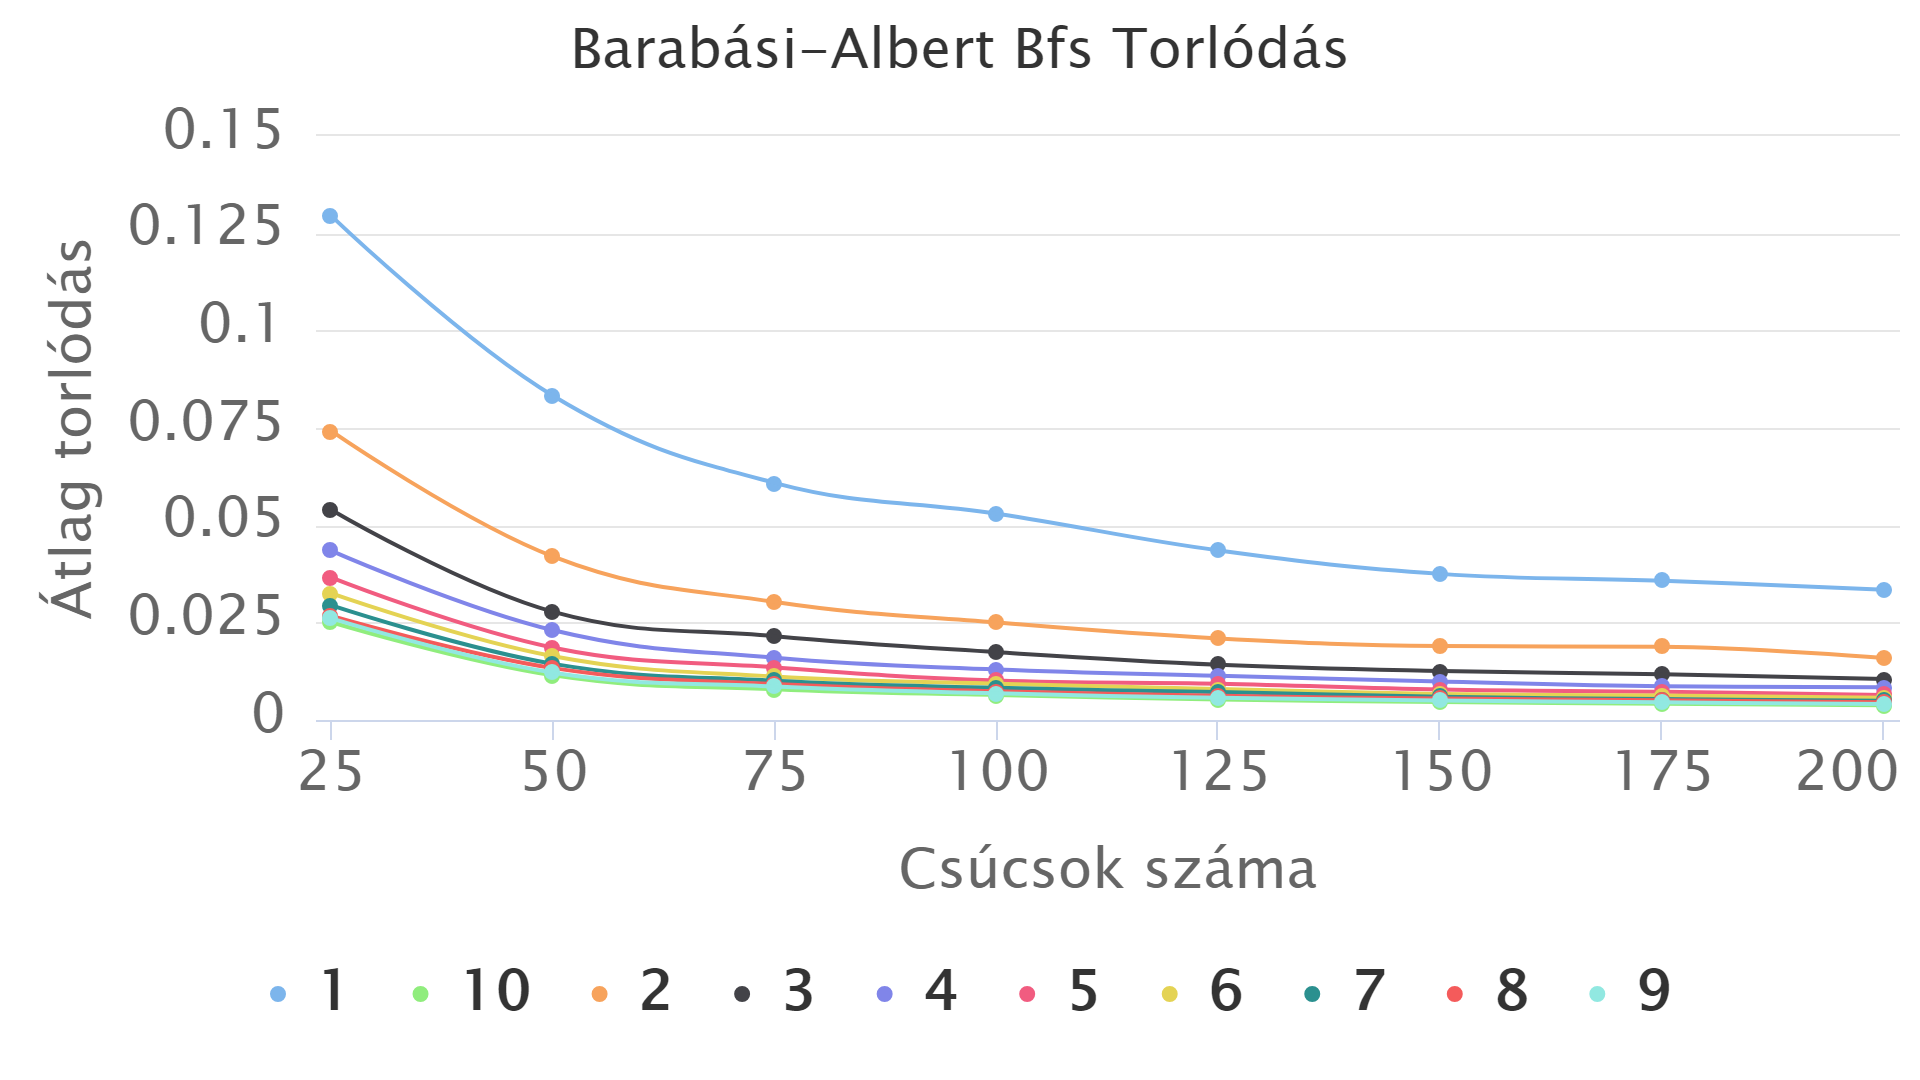
\includegraphics[width=0.49\linewidth]{pictures/barabasi_con_bfs.png}
		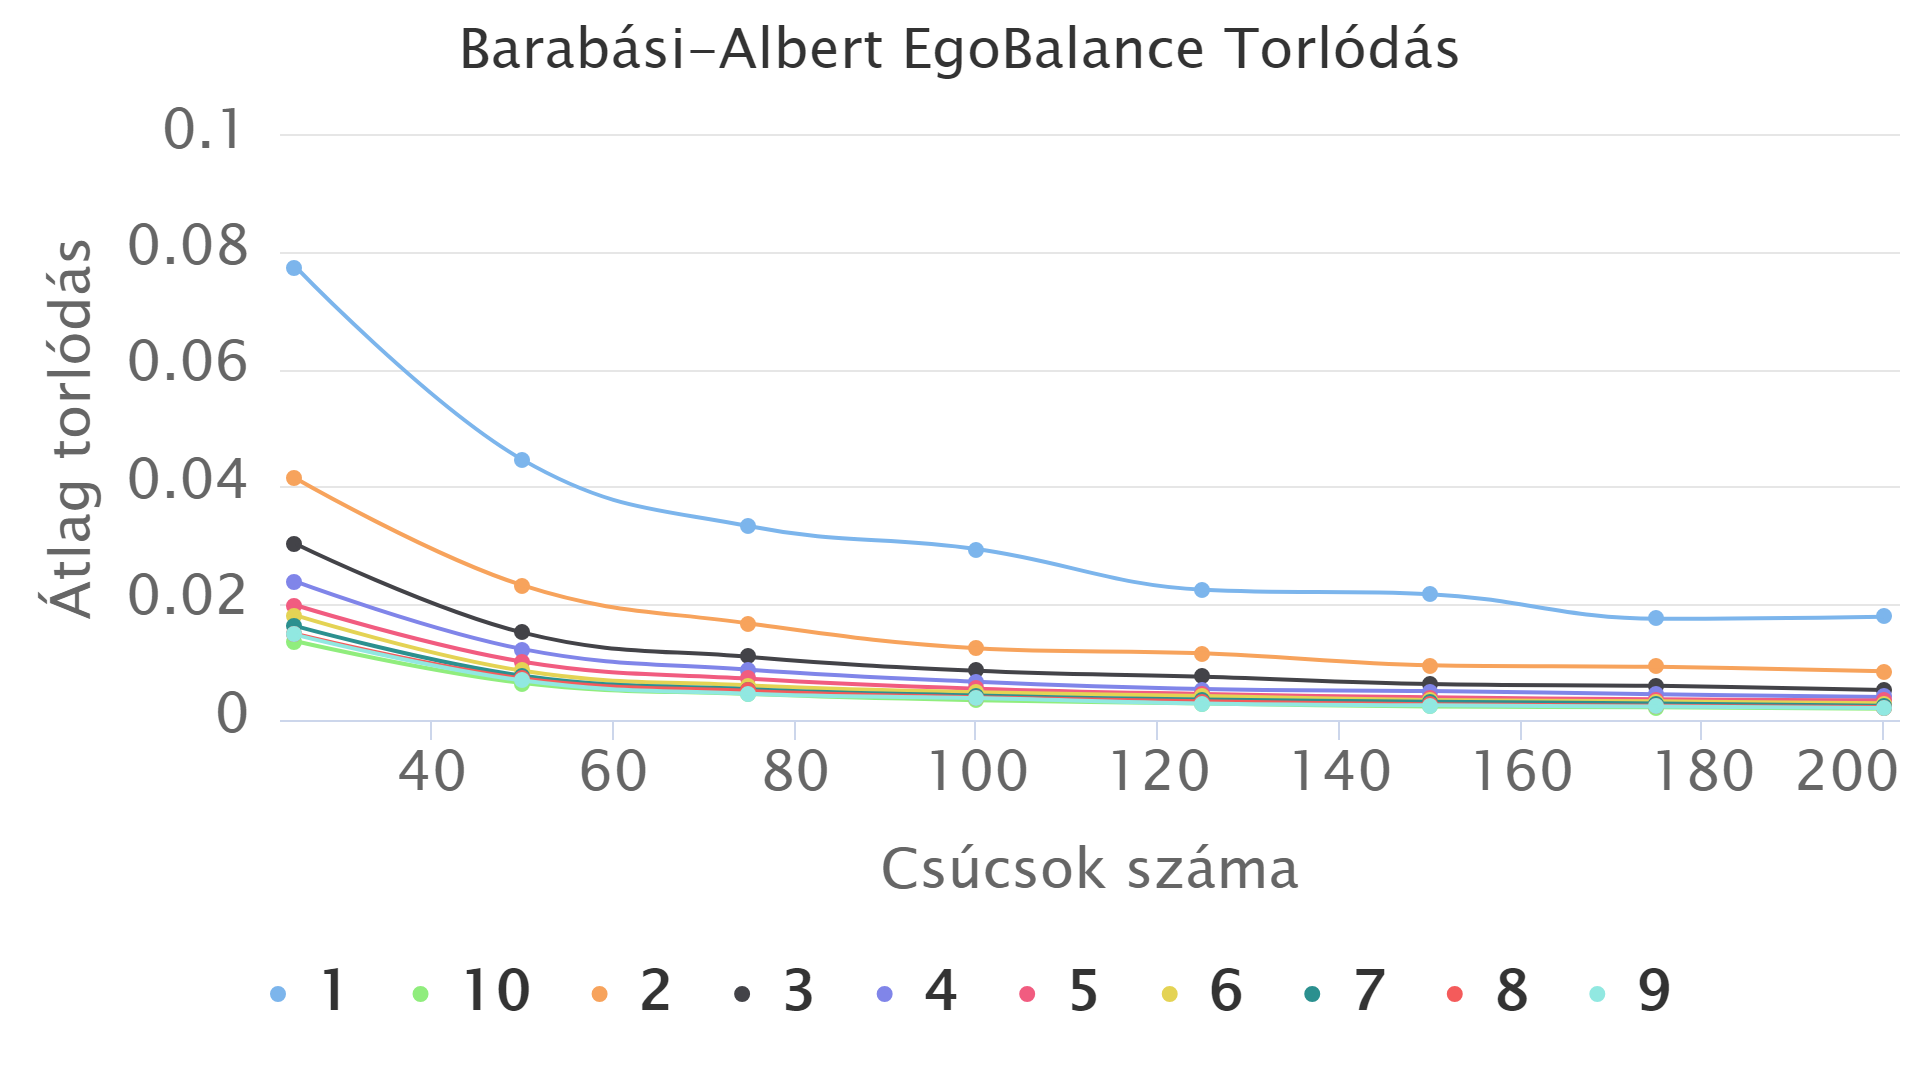
\includegraphics[width=0.49\linewidth]{pictures/barabasi_con_egobalance.png}
		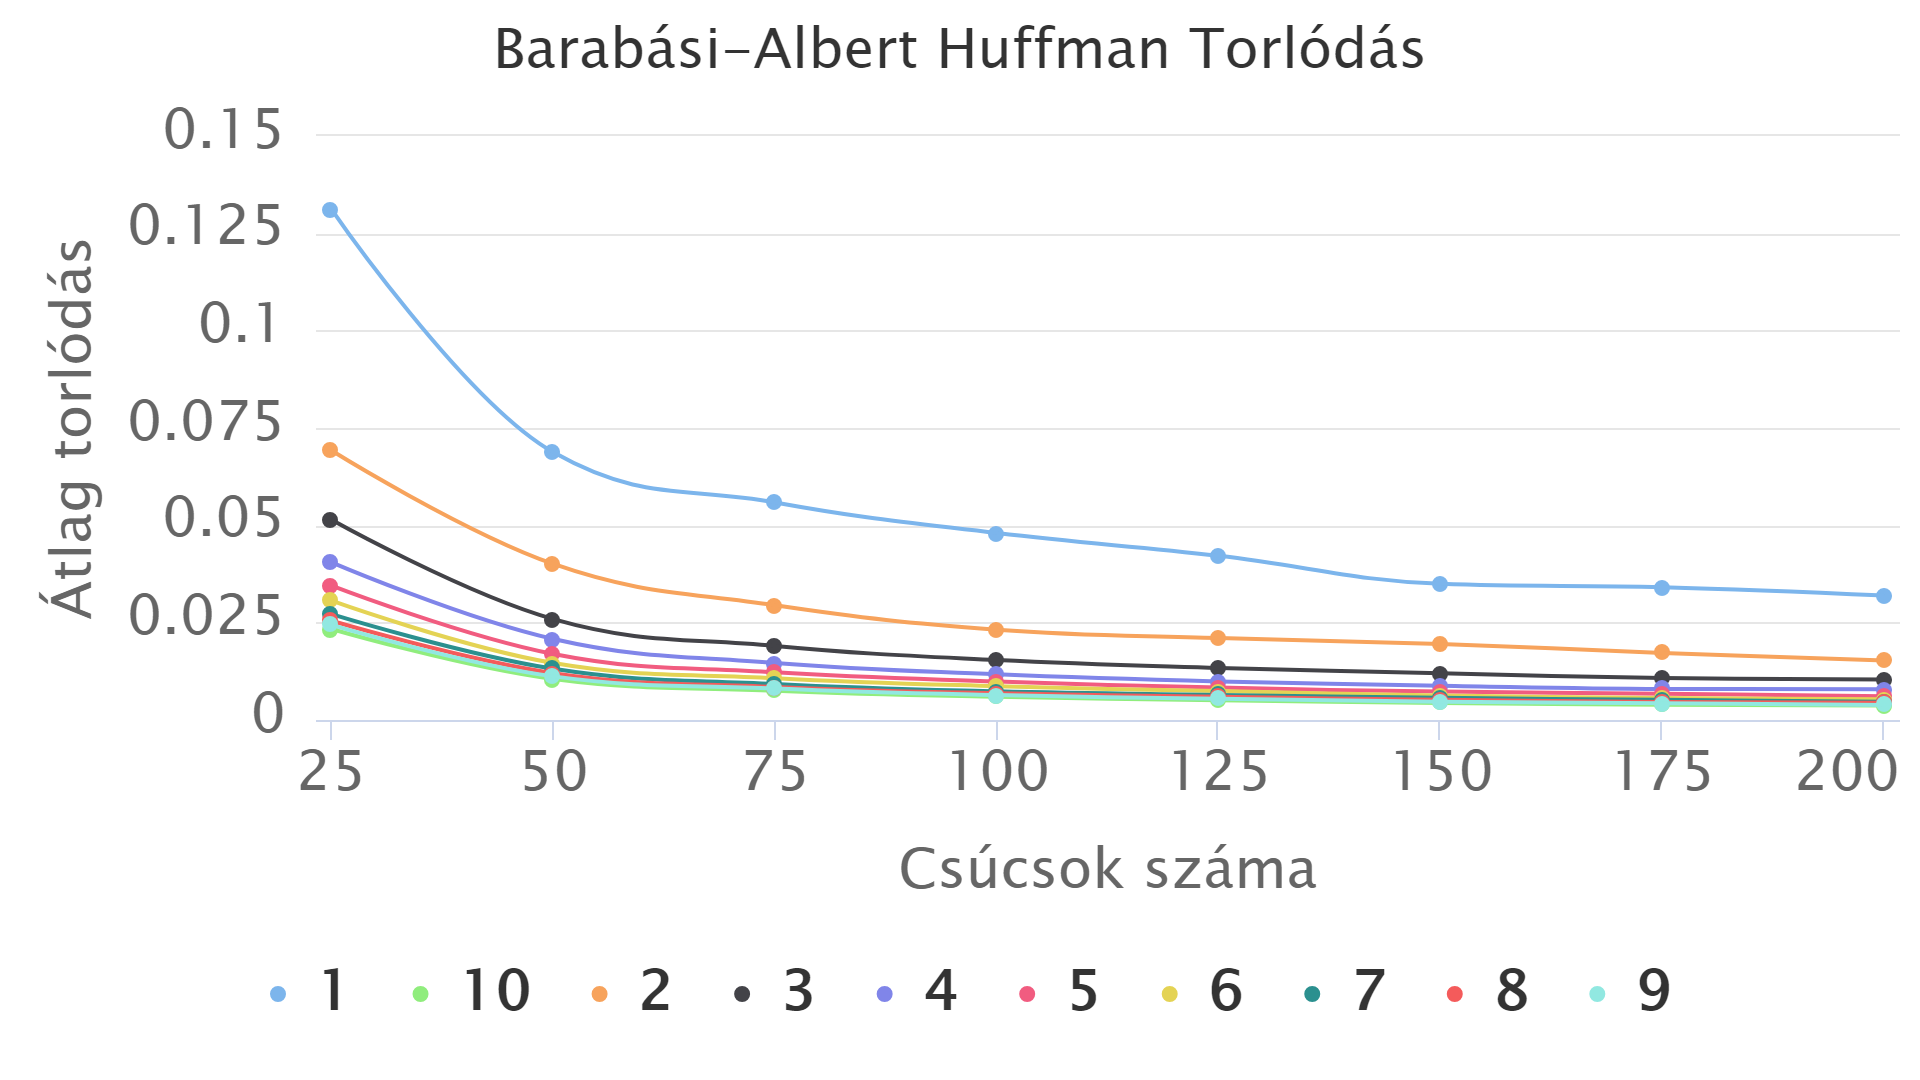
\includegraphics[width=0.49\linewidth]{pictures/barabasi_con_huffman.png}
		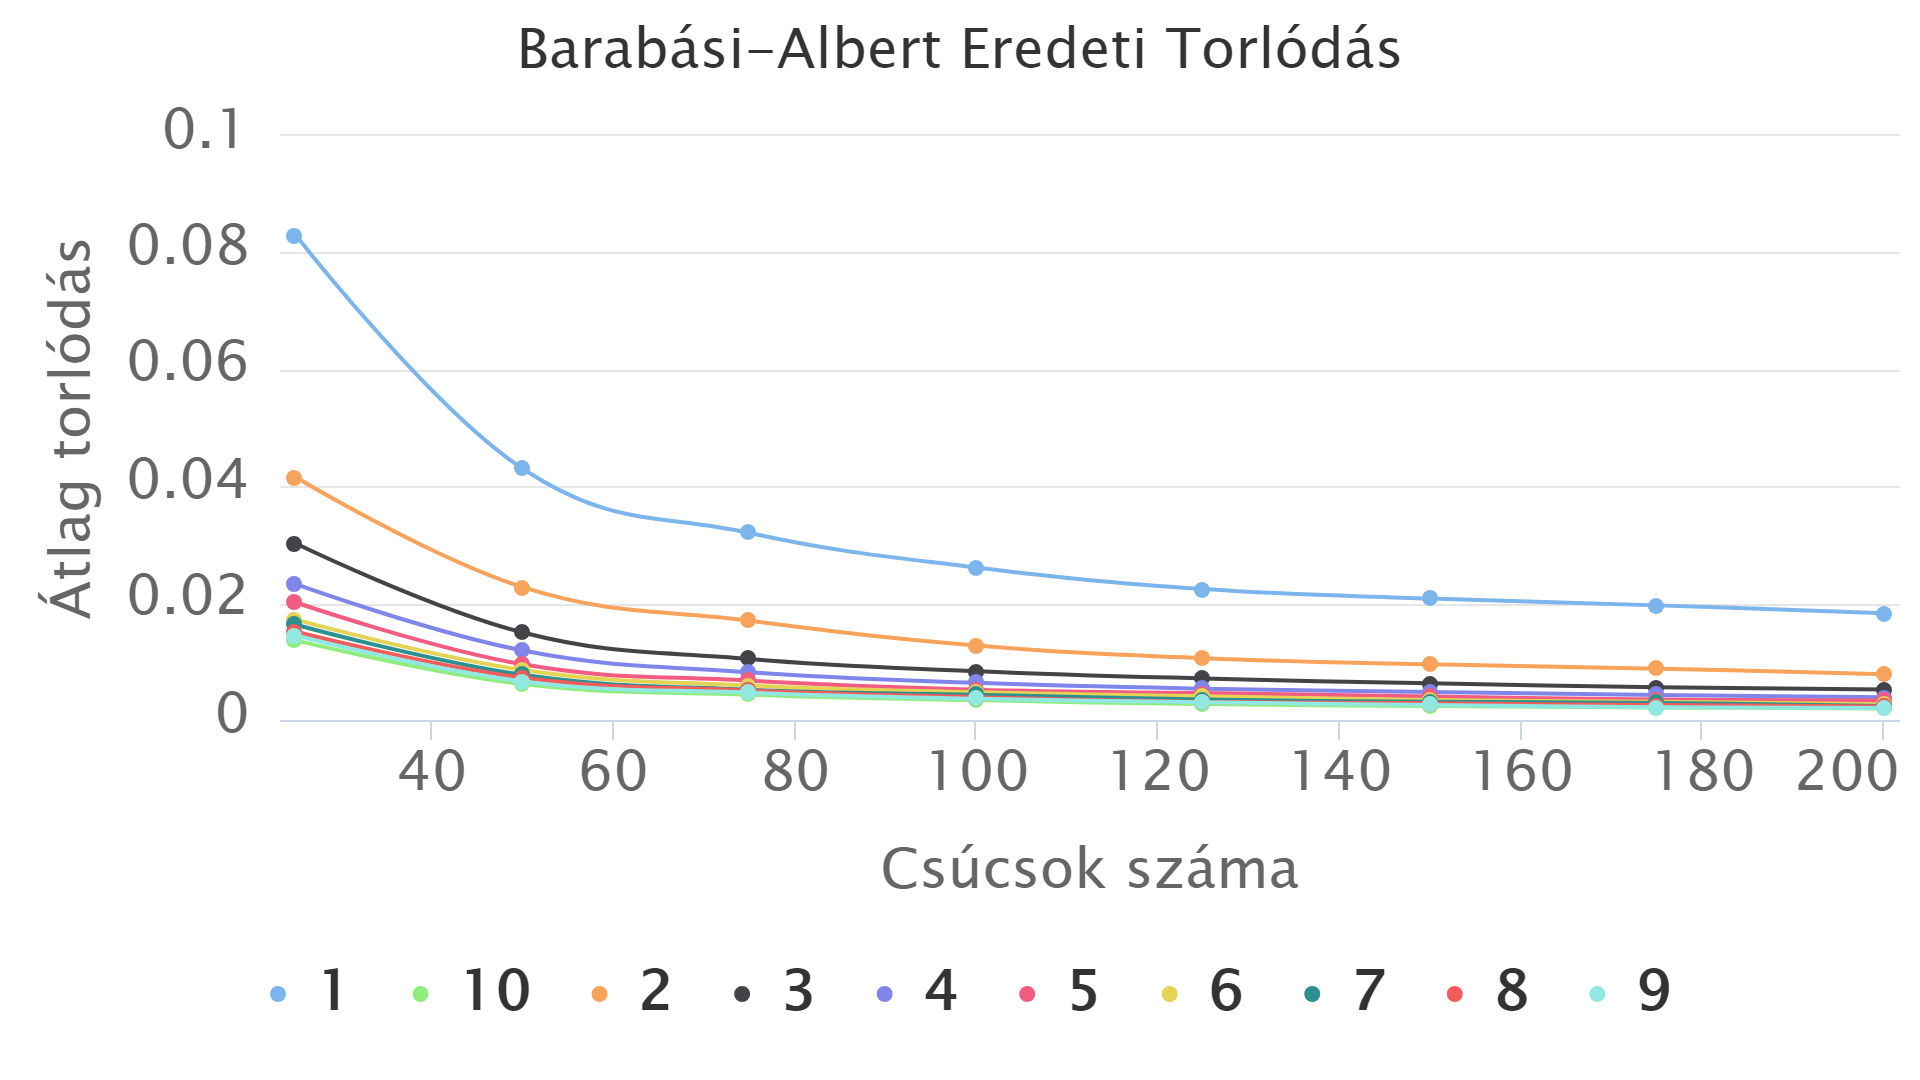
\includegraphics[width=0.49\linewidth]{pictures/barabasi_con_original.png}
		\caption{Átlag torlódás Barabási-Albert Gráf}
		\label{avg-len}
	\end{center}
\end{figure}


\begin{figure}[h]
	\begin{center}
		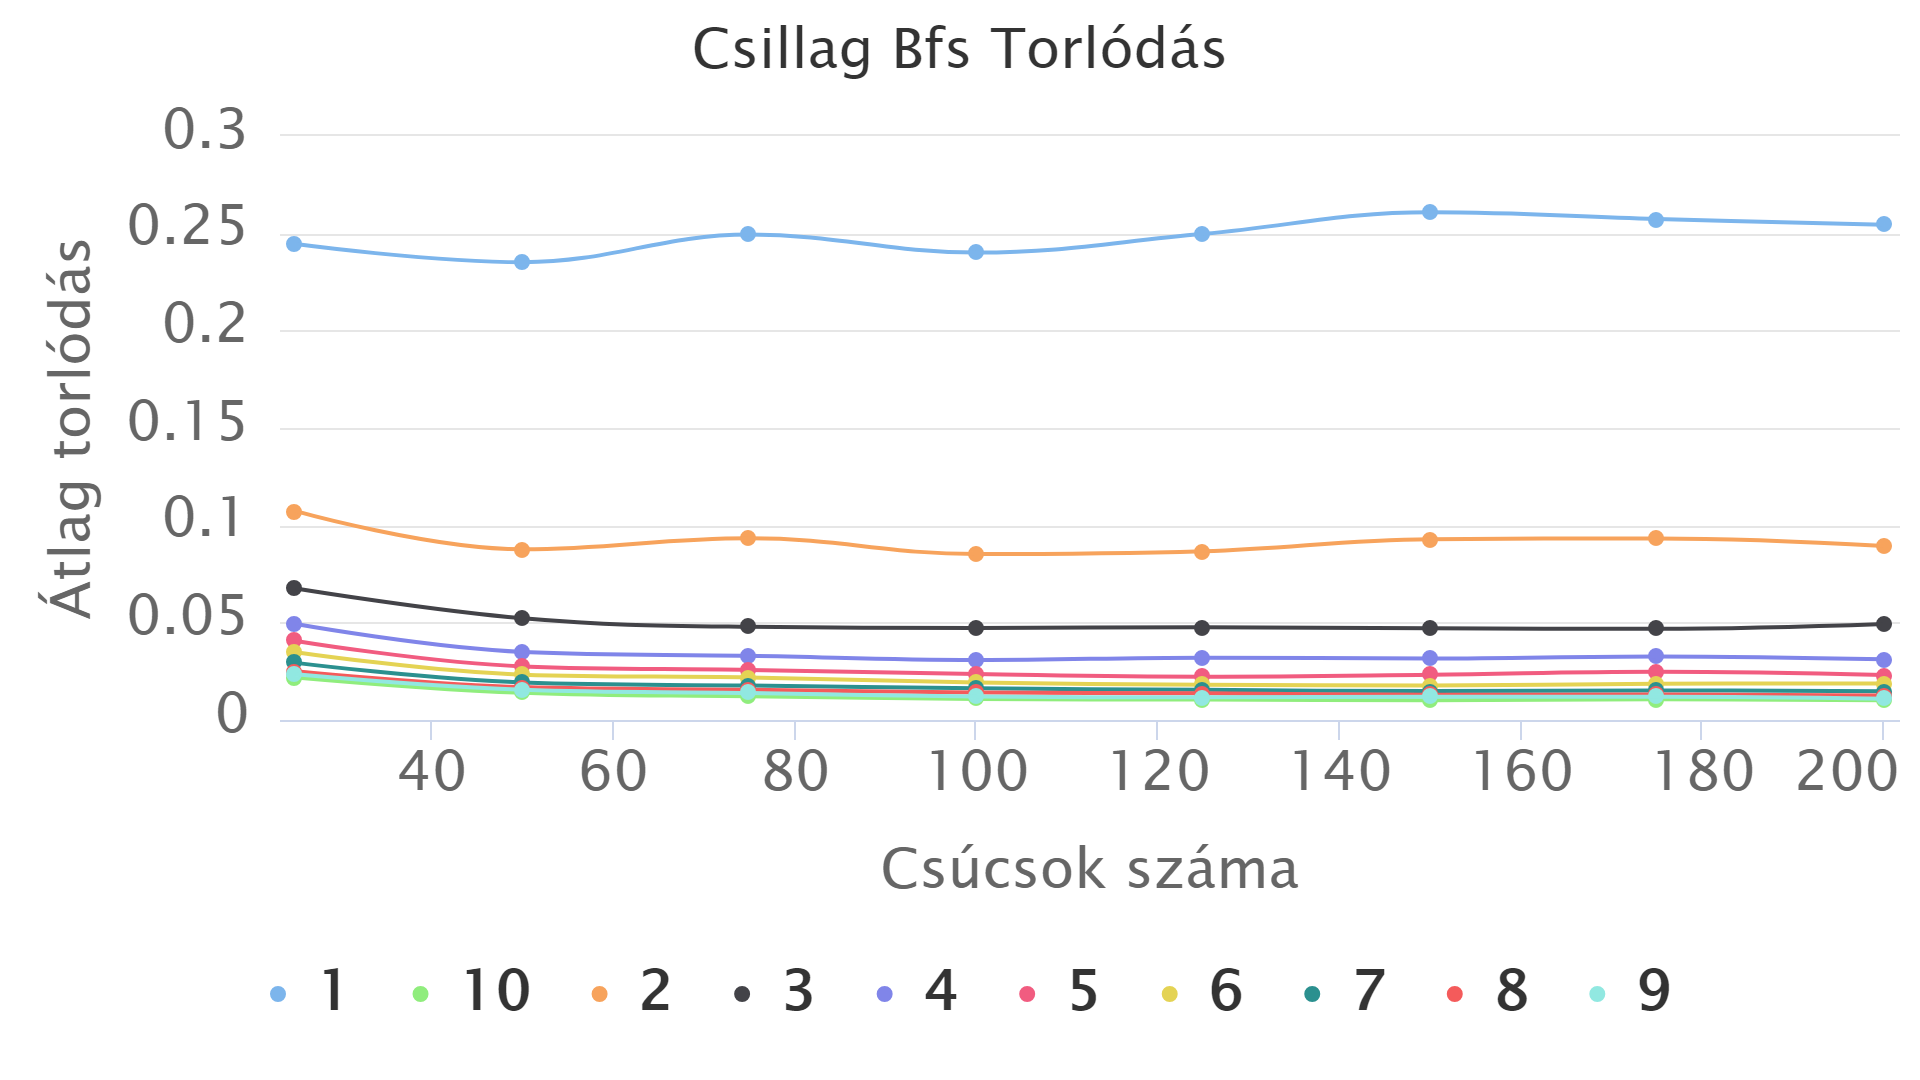
\includegraphics[width=0.49\linewidth]{pictures/star_con_bfs.png}
		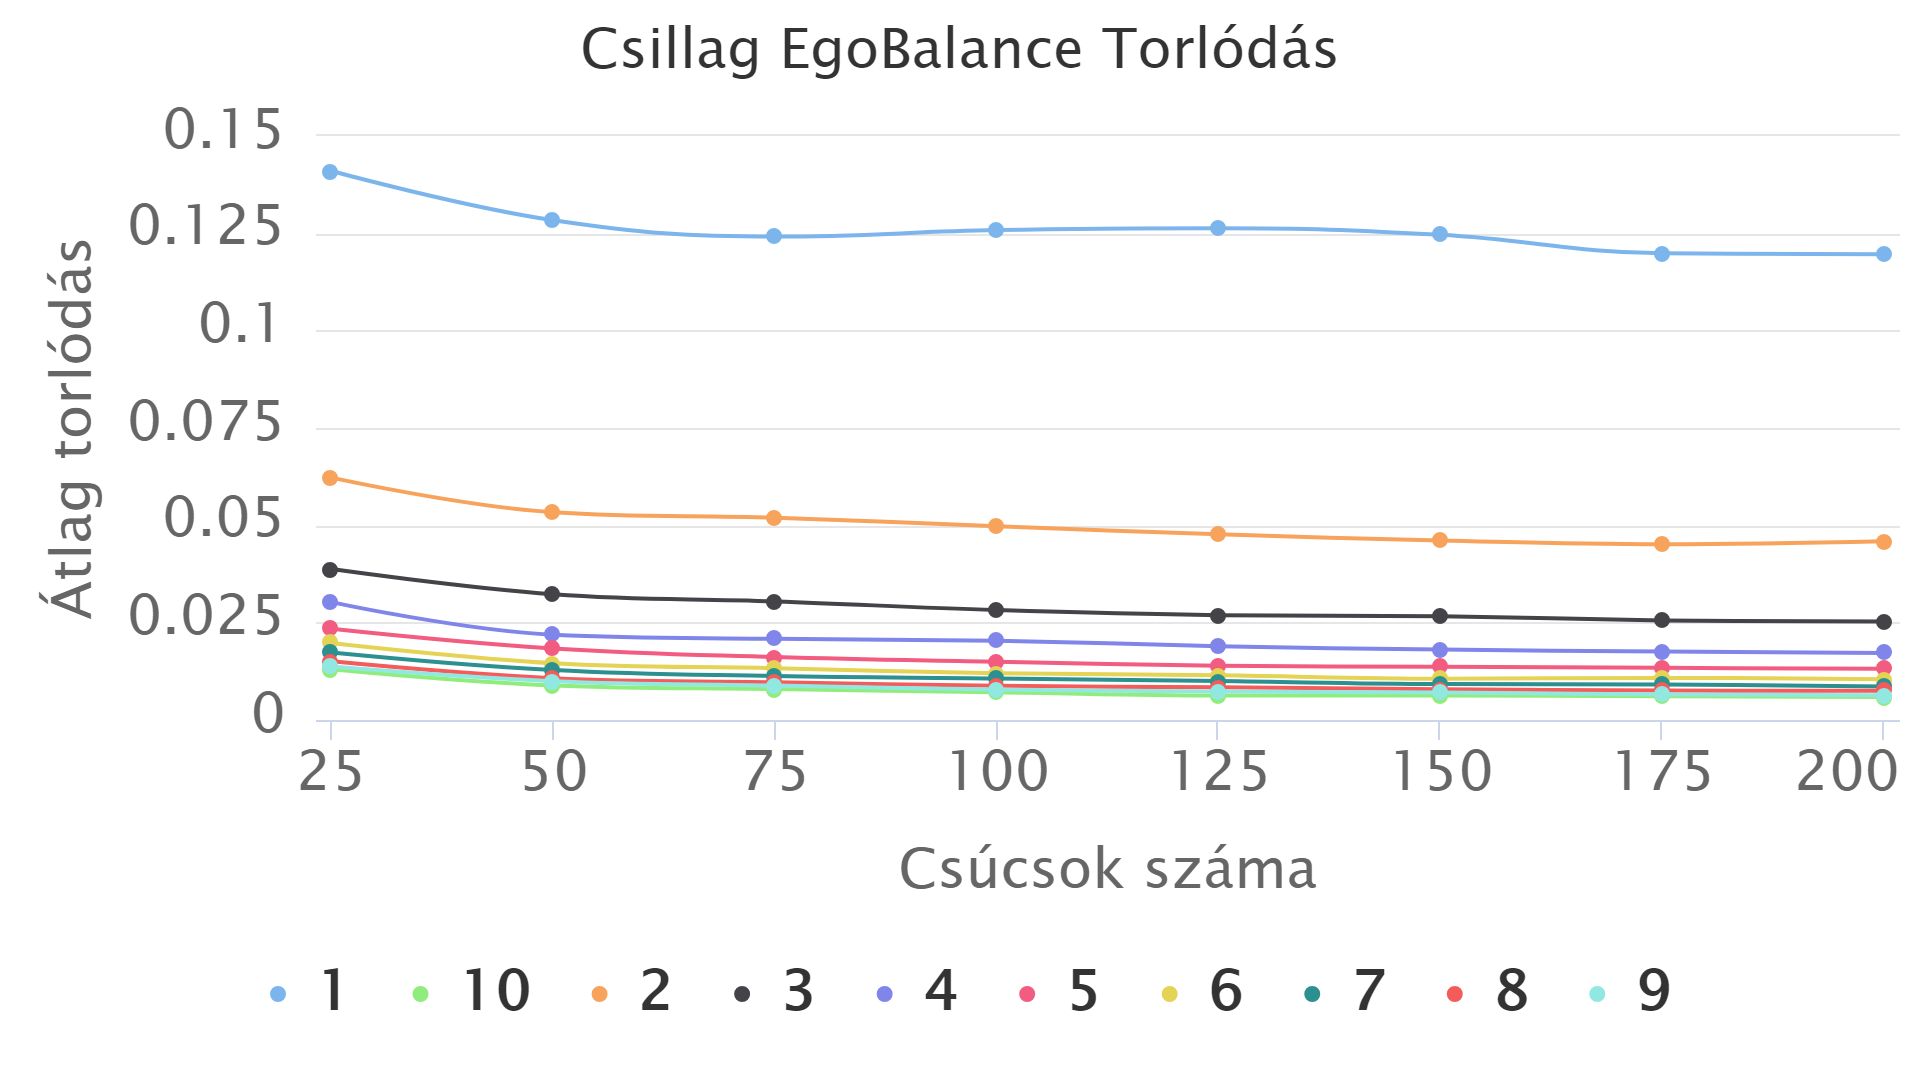
\includegraphics[width=0.49\linewidth]{pictures/star_con_egobalance.png}
		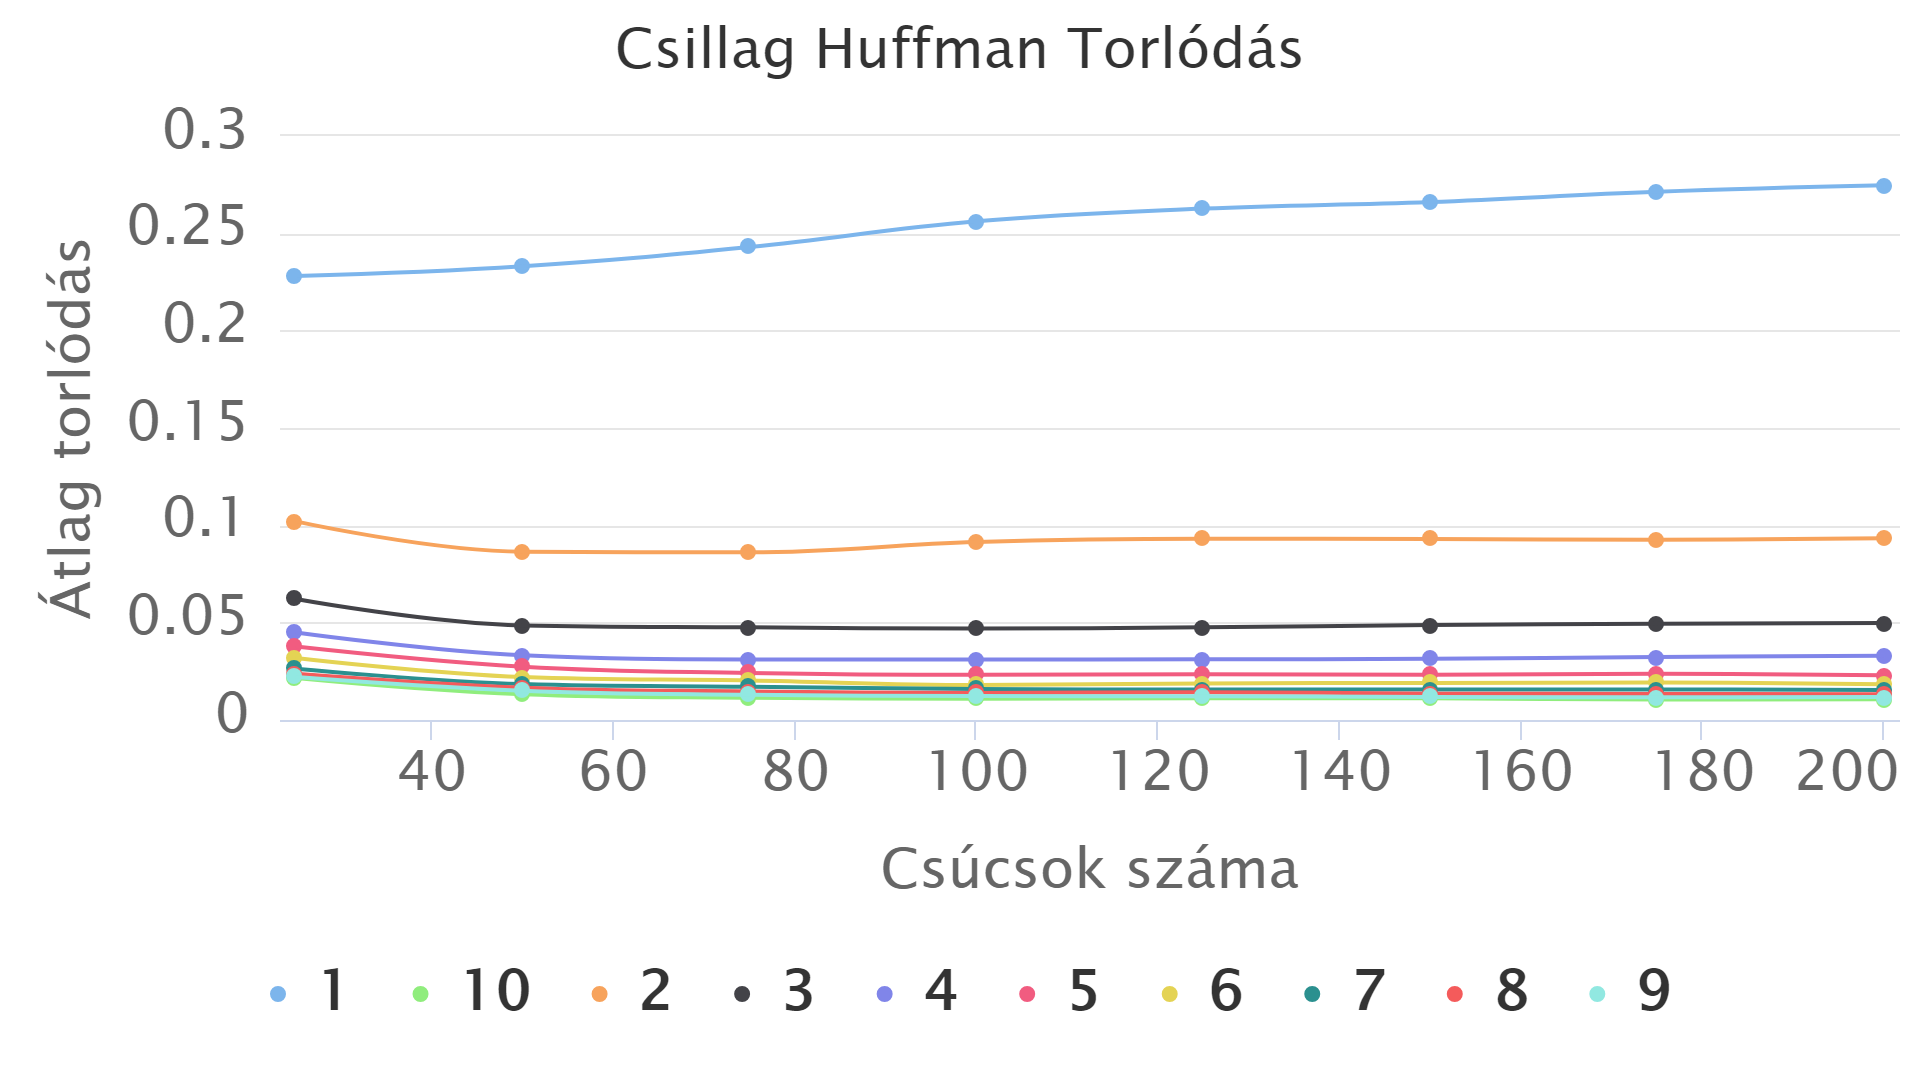
\includegraphics[width=0.49\linewidth]{pictures/star_con_huffman.png}
		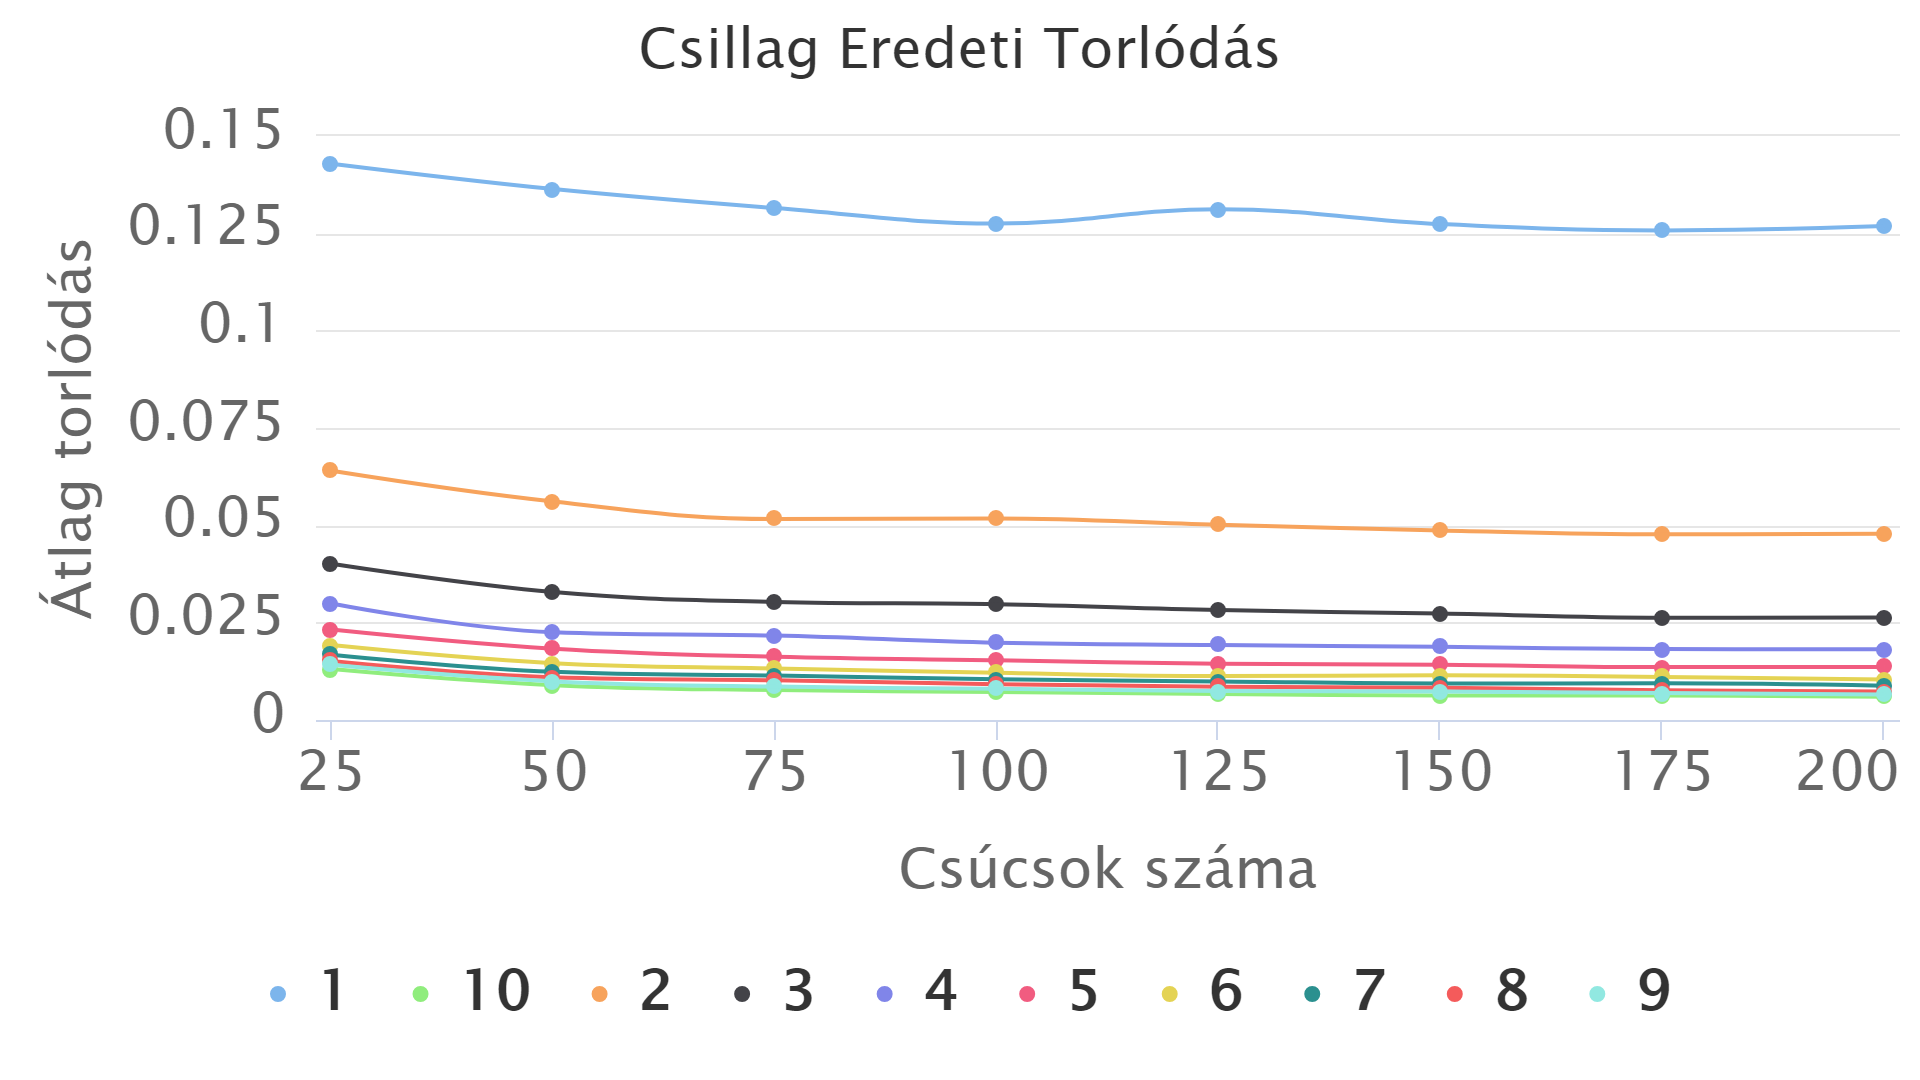
\includegraphics[width=0.49\linewidth]{pictures/star_con_original.png}
		\caption{Átlag torlódás Csillag Gráf}
		\label{avg-len}
	\end{center}
\end{figure}

\begin{figure}[h]
	\begin{center}
		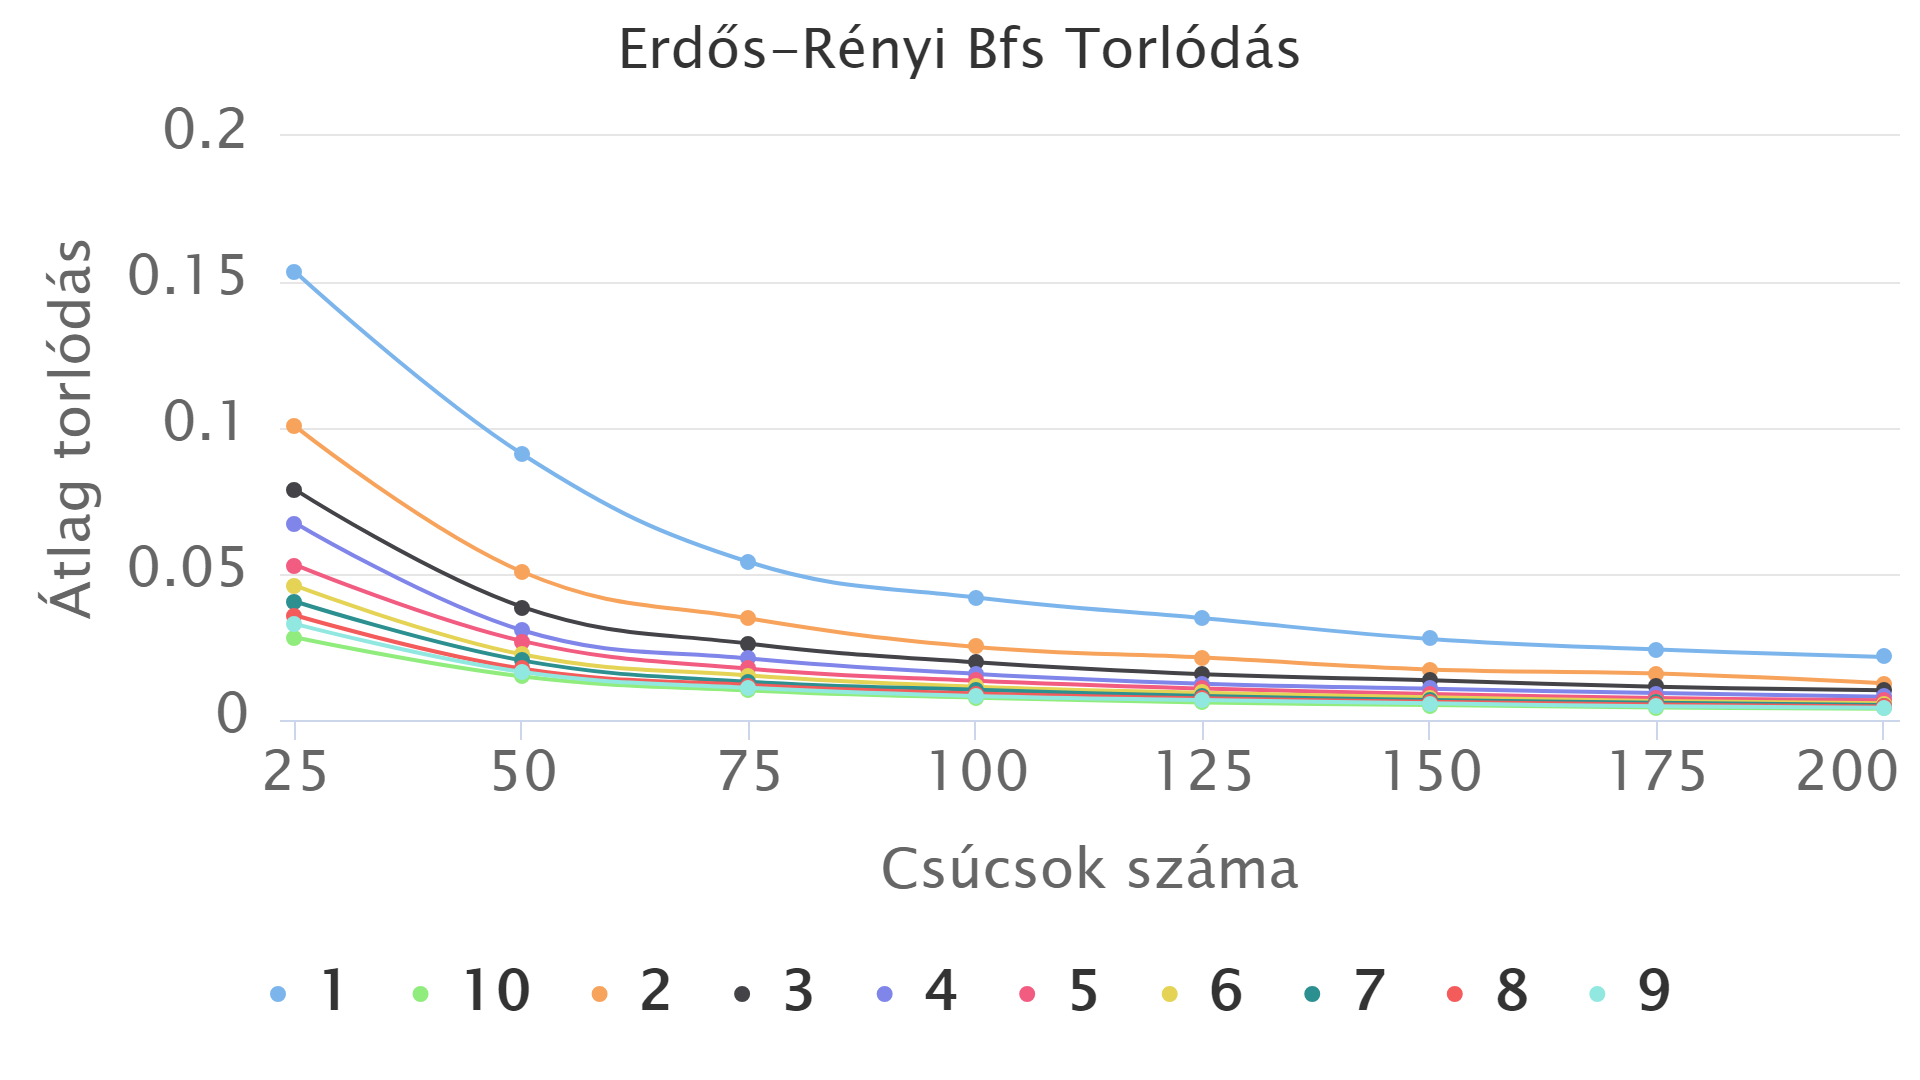
\includegraphics[width=0.49\linewidth]{pictures/erdos_con_bfs.png}
		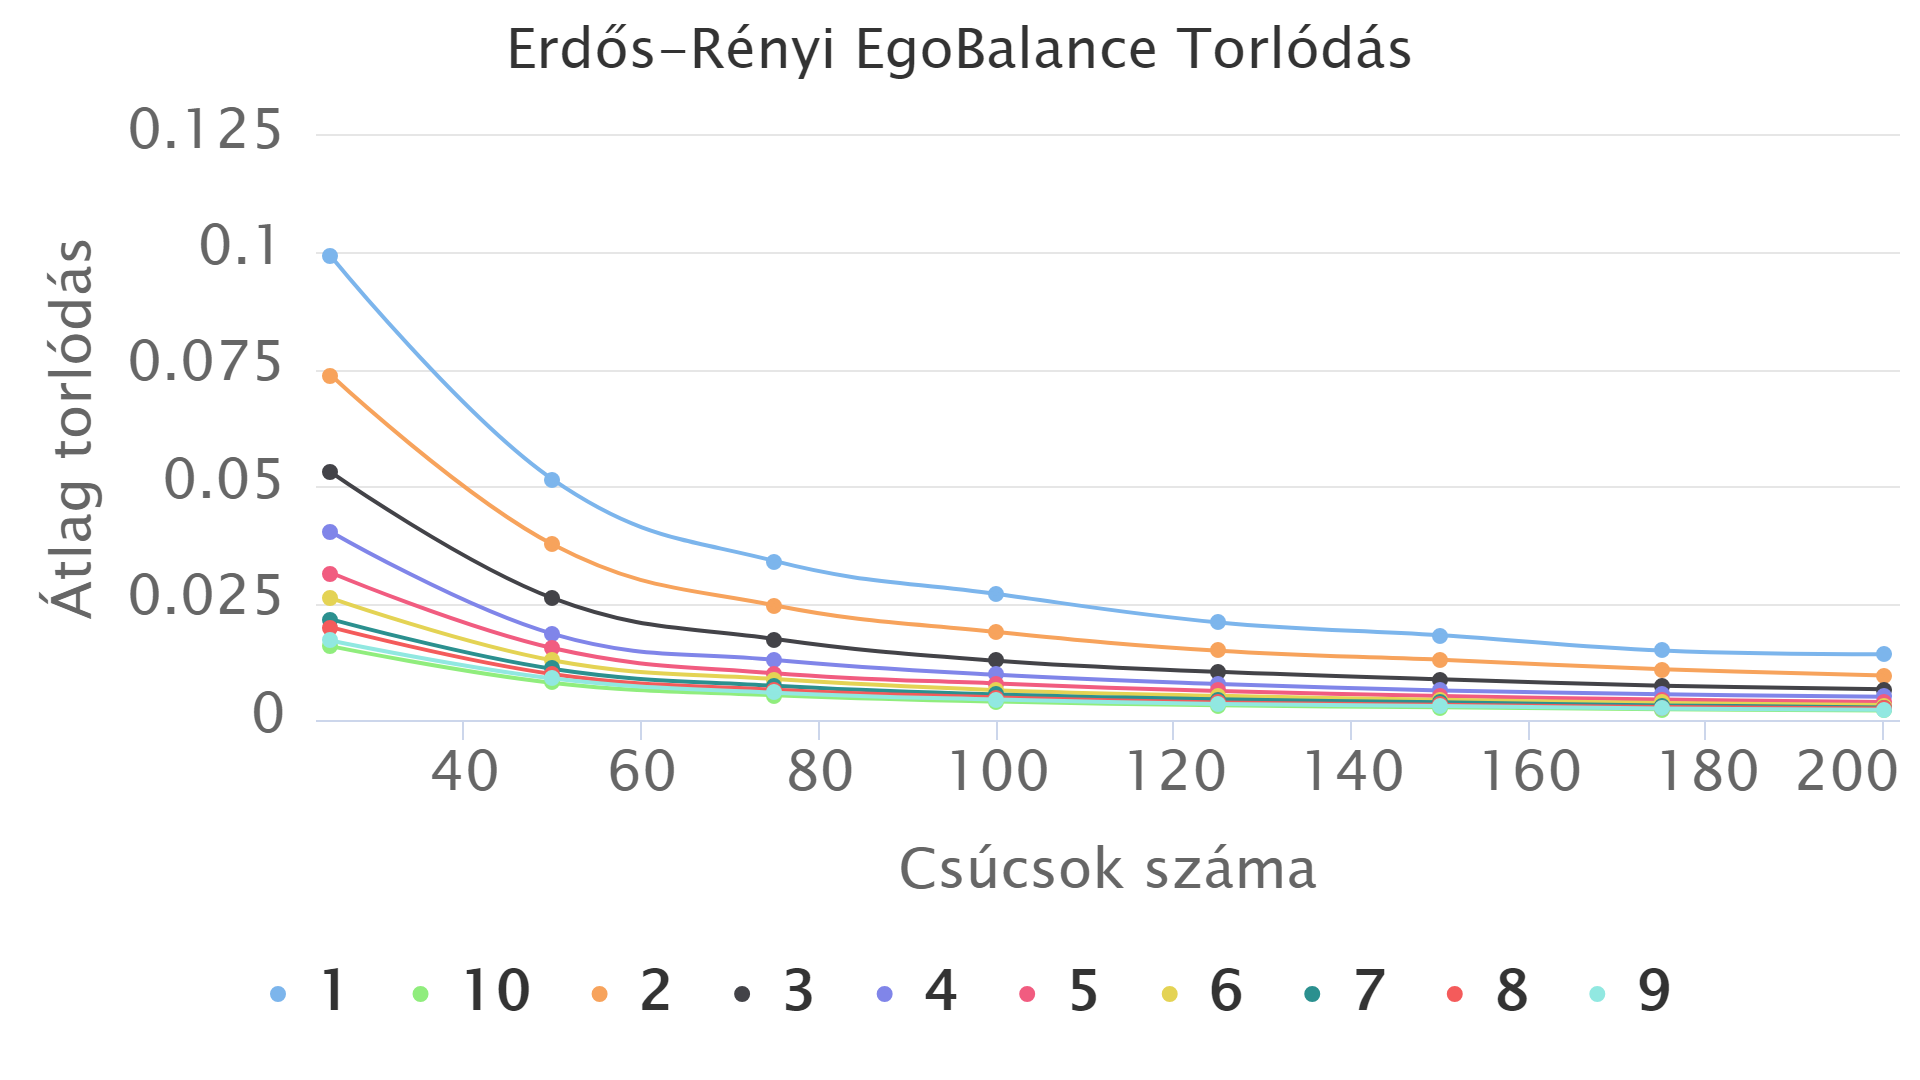
\includegraphics[width=0.49\linewidth]{pictures/erdos_con_egobalance.png}
		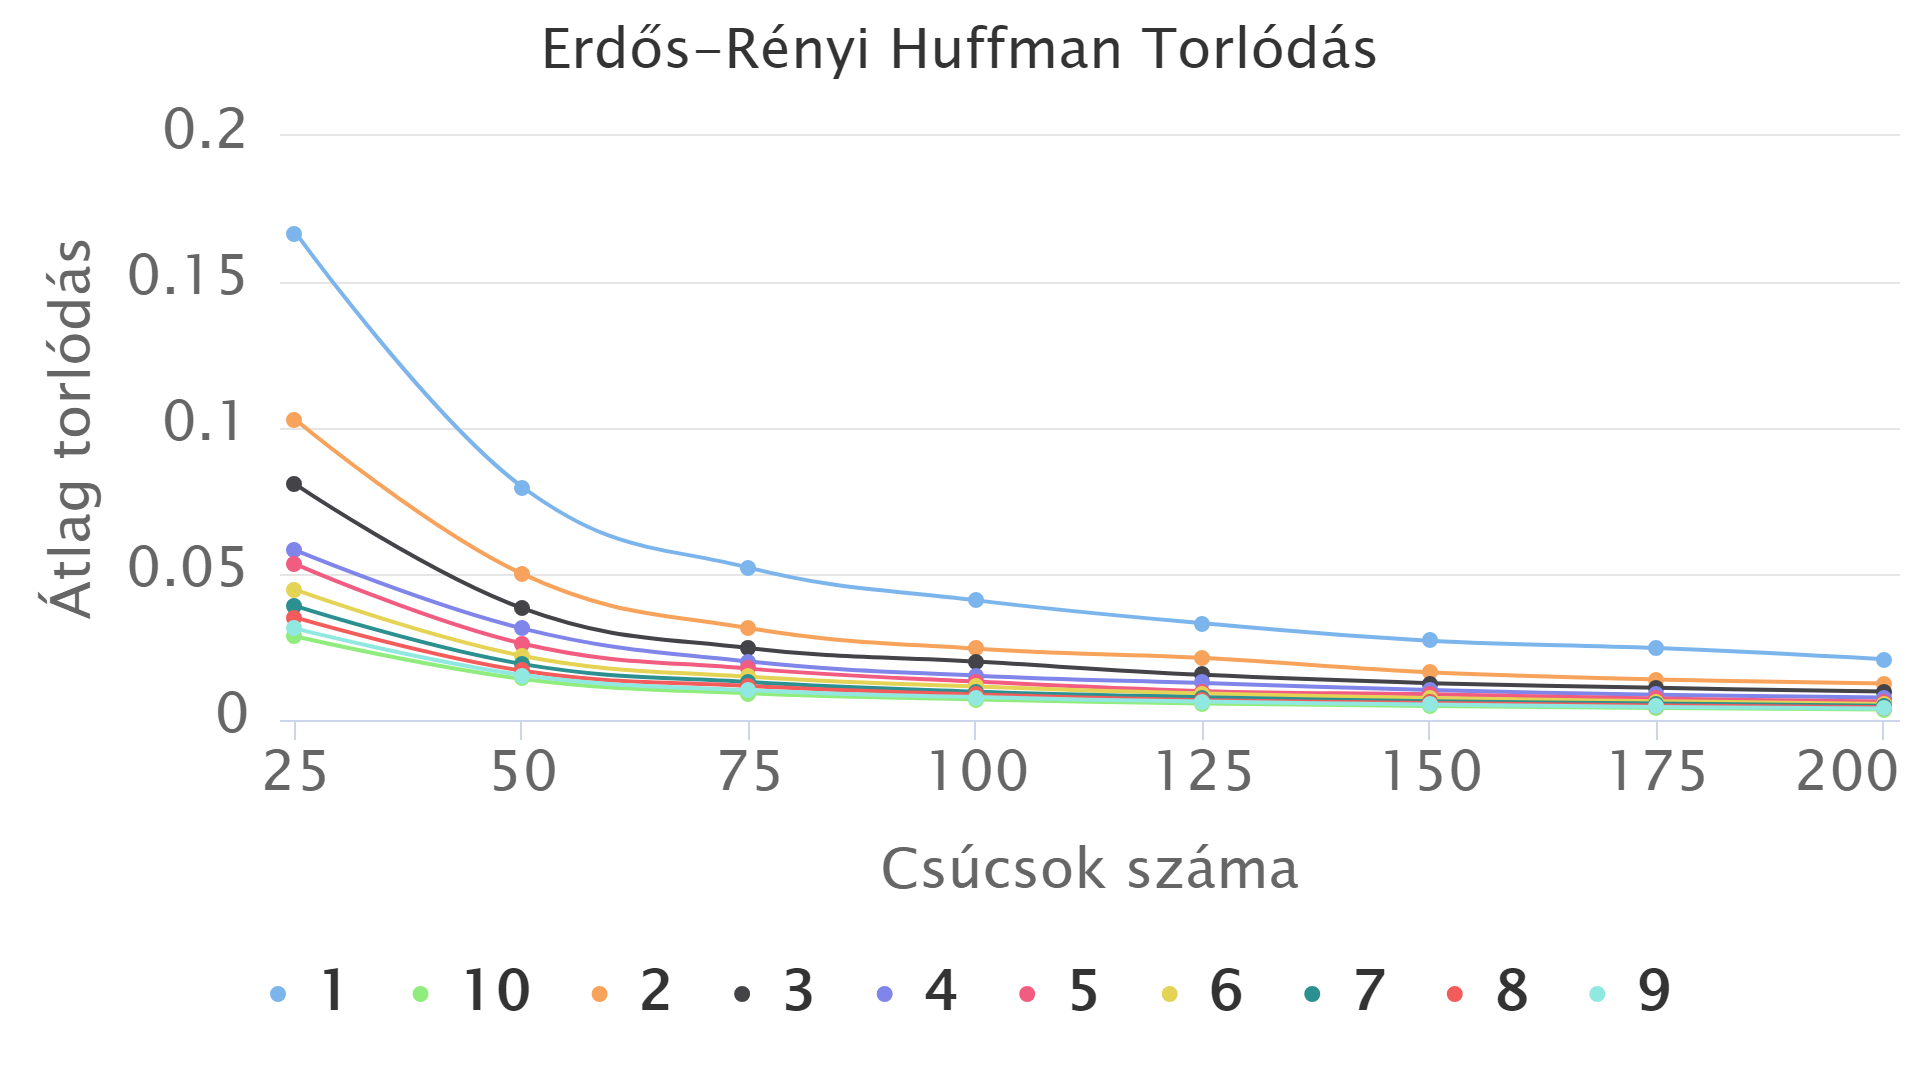
\includegraphics[width=0.49\linewidth]{pictures/erdos_con_huffman.png}
		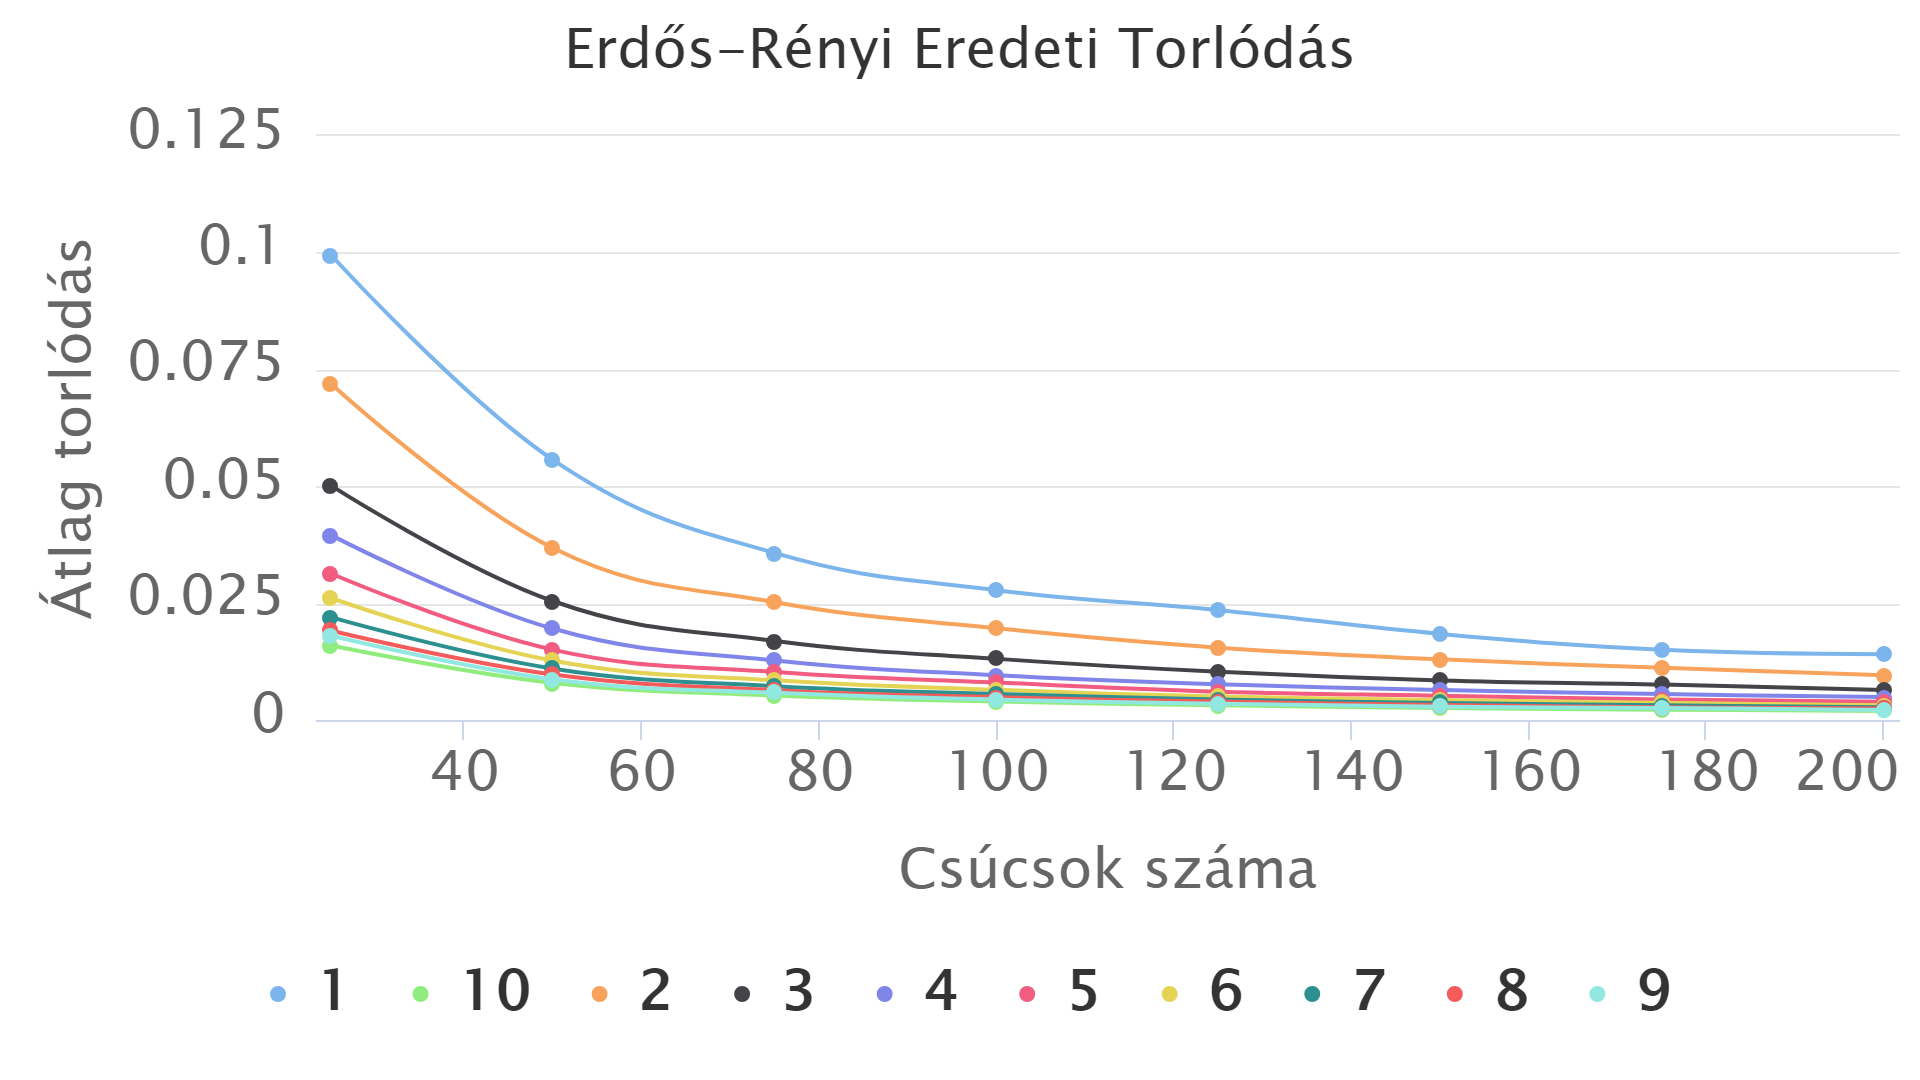
\includegraphics[width=0.49\linewidth]{pictures/erdos_con_original.png}
		\caption{Átlag torlódás Erdős-Rényi Gráf}
		\label{avg-len}
	\end{center}
\end{figure}



\chapter{Összefoglalás}

\section{Labor eredménye}

A tesztek kiértékelésének eredménye azt mutatja, hogy mind a négy algoritmus helytálló, mert hasonló eredményeket kapunk.
Az úthosszra nézve az algoritmusok teljesítménye nagyon hasonló, és benne van mérési hiba tartományában.
A torlódásra nézve van jelentős különbség.
A Huffman fa alapú algoritmusok nem veszik figyelembe a egyáltalán a torlódást, ezért nagyobb is határozottan bennük.
 
Két algoritmus ami hasonló módon építi fel a fát az a sorfolytonos (Bfs) és az EgoBalance. 
A kettő közötti lényeges különbség, amíg az EgoFa legnehezebbtől legkönnyebbig próbálja a legjobban elosztani a súlyokat, addig a sorfolytonos folyamatosan rakja fel őket.
Egy ilyen kis eltérés határozottan jobb eredményhez vezet az EgoFák esetén.

A végső összesítésből az látszik, hogy a szerzők által felvázolt EgoFa egy megfelelő adatszerkezet arra a célra, hogy hálózatot építünk vele.


\bibliographystyle{abbrv}
\bibliography{refrences}

	
\end{document}